%%
%% This is file `sample-sigconf.tex',
%% generated with the docstrip utility.
%%
%% The original source files were:
%%
%% samples.dtx  (with options: `sigconf')
%% 
%% IMPORTANT NOTICE:
%% 
%% For the copyright see the source file.
%% 
%% Any modified versions of this file must be renamed
%% with new filenames distinct from sample-sigconf.tex.
%% 
%% For distribution of the original source see the terms
%% for copying and modification in the file samples.dtx.
%% 
%% This generated file may be distributed as long as the
%% original source files, as listed above, are part of the
%% same distribution. (The sources need not necessarily be
%% in the same archive or directory.)
%%
%% The first command in your LaTeX source must be the \documentclass
%% command.
\documentclass[sigconf,review, anonymous]{acmart}
\acmConference[ESEC/FSE 2020]{The 28th ACM Joint European Software Engineering Conference and Symposium on the Foundations of Software Engineering}{8 - 13 November, 2020}{Sacramento, California, United States}

\pagenumbering{arabic} % Remove for camera-ready

\usepackage{subcaption}
\usepackage{libertine}
\usepackage{lipsum}% http://ctan.org/pkg/lipsum
\usepackage{algorithm}% http://ctan.org/pkg/algorithm
\usepackage{algpseudocode}% http://ctan.org/pkg/algorithmicx
\usepackage{graphicx}
\usepackage[compatibility=false]{caption}% http://ctan.org/pkg/caption
\usepackage{booktabs}
%% \usepackage{cite}
\usepackage{url}
\usepackage{multirow}
\usepackage{pgfplots}
\usepackage{tikz}
\usetikzlibrary{matrix,fit,shapes,calc,positioning,shadows,arrows,shapes,backgrounds,decorations.markings,fadings}
\usepgfplotslibrary{statistics}
\usepackage{listings}
%\usepackage[caption=false, font=footnotesize]{subfig}
\renewcommand{\ttdefault}{pcr}
\lstset{
  basicstyle=\scriptsize\ttfamily,
  keywordstyle=\scriptsize\ttfamily\bfseries,
  language=C,             % choose the language of the code
  frame=single,              % adds a frame around the code
  aboveskip=0pt,
  belowskip=0pt,
  breaklines=true,           % sets automatic line breaking
  breakatwhitespace=true,   % sets if automatic breaks should only happen at
  showspaces=false,
  %numbersep=5pt,              % Abstand der Nummern zum Text
  %tabsize=2,                  % Groesse von Tabs
  %extendedchars=true,         %
  keywords=[2]{tcp, flag, threshold, track, count, seconds, classtype, sid}
}
\usepackage{balance}
\usepackage{wrapfig}
\usepackage{enumitem}
\usepackage{color, colortbl}
\definecolor{Gray}{gray}{0.9}
\usepackage[skins]{tcolorbox}

%% 
\newcommand{\tname}{\textsc{Syrius}} %% name of the technique
\newcommand{\ie}{i.e.}
\newcommand{\eg}{e.g.}
\newcommand{\aka}{a.k.a.}
\newcommand{\etal}{and colleagues}
\newcommand{\nids}{NIDS}
\newcommand{\metas}{Metasploit}
\newcommand{\suri}{Suricata}
\newcommand{\numrulessuri}{27.8K}
\newcommand{\percRulesWithContent}{93.5\%}
\newcommand{\numundetected}{\Fix{XX\%}}
\newcommand{\CodeIn}[1]{{\small{\texttt{#1}}}}
\newcommand{\MyComment}[1]{}

%% review
\newcommand{\Fix}[1]{{\textbf{[[}\color{magenta}#1}\textbf{]]}}
\newcommand{\Mar}[1]{{\textbf{[[Marcelo:~}\color{red}#1}\textbf{]]}}
\newcommand{\Luc}[1]{{\textbf{[[Lucas:~}\color{blue}#1}\textbf{]]}}
\newcommand{\Gui}[1]{{\textbf{[[Guilherme:~}\color{green}#1}\textbf{]]}}

\def\denseitems{
   \itemsep1pt plus1pt minus1pt
   \parsep0pt plus0pt
   \parskip0pt\topsep0pt}

%% numbers
\newcommand{\totoptions}{162}
\newcommand{\numproto}{11}
\newcommand{\totoptionsrelevant}{153}


%%
%% \BibTeX command to typeset BibTeX logo in the docs
\AtBeginDocument{%
  \providecommand\BibTeX{{%
    \normalfont B\kern-0.5em{\scshape i\kern-0.25em b}\kern-0.8em\TeX}}}

%% Rights management information.  This information is sent to you
%% when you complete the rights form.  These commands have SAMPLE
%% values in them; it is your responsibility as an author to replace
%% the commands and values with those provided to you when you
%% complete the rights form.
%% \setcopyright{acmcopyright}
%% \copyrightyear{2018}
%% \acmYear{2018}
%% \acmDOI{10.1145/1122445.1122456}

%% These commands are for a PROCEEDINGS abstract or paper.
%% \acmConference[Woodstock '18]{Woodstock '18: ACM Symposium on Neural
%%   Gaze Detection}{June 03--05, 2018}{Woodstock, NY}
%% \acmBooktitle{Woodstock '18: ACM Symposium on Neural Gaze Detection,
%%   June 03--05, 2018, Woodstock, NY}
%% \acmPrice{15.00}
%% \acmISBN{978-1-4503-XXXX-X/18/06}


%%
%% Submission ID.
%% Use this when submitting an article to a sponsored event. You'll
%% receive a unique submission ID from the organizers
%% of the event, and this ID should be used as the parameter to this command.
%%\acmSubmissionID{123-A56-BU3}

%%
%% The majority of ACM publications use numbered citations and
%% references.  The command \citestyle{authoryear} switches to the
%% "author year" style.
%%
%% If you are preparing content for an event
%% sponsored by ACM SIGGRAPH, you must use the "author year" style of
%% citations and references.
%% Uncommenting
%% the next command will enable that style.
%%\citestyle{acmauthoryear}

%%
%% end of the preamble, start of the body of the document source.
\begin{document}

%%
%% The "title" command has an optional parameter,
%% allowing the author to define a "short title" to be used in page headers.
\title{Learning to Synthesize Rules for Rule-based Intrusion Detectors}

%%
%% The "author" command and its associated commands are used to define
%% the authors and their affiliations.
%% Of note is the shared affiliation of the first two authors, and the
%% "authornote" and "authornotemark" commands
%% used to denote shared contribution to the research.
\author{Ben Trovato}
\authornote{Both authors contributed equally to this research.}
\email{trovato@corporation.com}
\orcid{1234-5678-9012}
\author{G.K.M. Tobin}
\authornotemark[1]
\email{webmaster@marysville-ohio.com}
\affiliation{%
  \institution{Institute for Clarity in Documentation}
  \streetaddress{P.O. Box 1212}
  \city{Dublin}
  \state{Ohio}
  \postcode{43017-6221}
}

\author{Lars Th{\o}rv{\"a}ld}
\affiliation{%
  \institution{The Th{\o}rv{\"a}ld Group}
  \streetaddress{1 Th{\o}rv{\"a}ld Circle}
  \city{Hekla}
  \country{Iceland}}
\email{larst@affiliation.org}

\author{Valerie B\'eranger}
\affiliation{%
  \institution{Inria Paris-Rocquencourt}
  \city{Rocquencourt}
  \country{France}
}

\author{Aparna Patel}
\affiliation{%
 \institution{Rajiv Gandhi University}
 \streetaddress{Rono-Hills}
 \city{Doimukh}
 \state{Arunachal Pradesh}
 \country{India}}

\author{Huifen Chan}
\affiliation{%
  \institution{Tsinghua University}
  \streetaddress{30 Shuangqing Rd}
  \city{Haidian Qu}
  \state{Beijing Shi}
  \country{China}}

\author{Charles Palmer}
\affiliation{%
  \institution{Palmer Research Laboratories}
  \streetaddress{8600 Datapoint Drive}
  \city{San Antonio}
  \state{Texas}
  \postcode{78229}}
\email{cpalmer@prl.com}

\author{John Smith}
\affiliation{\institution{The Th{\o}rv{\"a}ld Group}}
\email{jsmith@affiliation.org}

\author{Julius P. Kumquat}
\affiliation{\institution{The Kumquat Consortium}}
\email{jpkumquat@consortium.net}

%%
%% By default, the full list of authors will be used in the page
%% headers. Often, this list is too long, and will overlap
%% other information printed in the page headers. This command allows
%% the author to define a more concise list
%% of authors' names for this purpose.
\renewcommand{\shortauthors}{Trovato and Tobin, et al.}

%%
%% The abstract is a short summary of the work to be presented in the
%% article.
\begin{abstract}
  \Fix{revise}
Network Intrusion Detection Systems (\nids{}) are a popular mechanism
used by system administrators to defend against network attacks. These
systems monitor the network traffic and flag suspicious network
behavior. Signature-based \nids\ do that by checking the\MyComment{ network}
traffic against a pre-defined set of rules, which become obsolete
as attackers learn new strategies to circumvent existing defenses.

This paper proposes \tname{}, a technique that automatically
synthesizes \nids\ rules from positive and negative examples, \ie{},
malicious and benign traffic. \tname{} formulates synthesis as an
optimization problem whose candidate solutions are rules. Optimal
solutions maximize the capture of positive traffic and minimize the
capture of negative traffic. \tname{} bootstraps the search with a
candidate solution inferred from the payload of the malicious message.
It uses that initial overfitting solution to search for alternative
rules that only capture the malicious traffic. Then, it ranks those
rules according to heuristics---drawn from a data set of existing
rules---denoting the likelihood of those rules of being useful.

We evaluated \tname{} on a diverse
set of attacks. Results indicate that \Fix{...}
\end{abstract}

%%
%% The code below is generated by the tool at http://dl.acm.org/ccs.cfm.
%% Please copy and paste the code instead of the example below.
%%
\begin{CCSXML}
<ccs2012>
 <concept>
  <concept_id>10010520.10010553.10010562</concept_id>
  <concept_desc>Computer systems organization~Embedded systems</concept_desc>
  <concept_significance>500</concept_significance>
 </concept>
 <concept>
  <concept_id>10010520.10010575.10010755</concept_id>
  <concept_desc>Computer systems organization~Redundancy</concept_desc>
  <concept_significance>300</concept_significance>
 </concept>
 <concept>
  <concept_id>10010520.10010553.10010554</concept_id>
  <concept_desc>Computer systems organization~Robotics</concept_desc>
  <concept_significance>100</concept_significance>
 </concept>
 <concept>
  <concept_id>10003033.10003083.10003095</concept_id>
  <concept_desc>Networks~Network reliability</concept_desc>
  <concept_significance>100</concept_significance>
 </concept>
</ccs2012>
\end{CCSXML}

\ccsdesc[500]{Computer systems organization~Embedded systems}
\ccsdesc[300]{Computer systems organization~Redundancy}
\ccsdesc{Computer systems organization~Robotics}
\ccsdesc[100]{Networks~Network reliability}

%%
%% Keywords. The author(s) should pick words that accurately describe
%% the work being presented. Separate the keywords with commas.
% \keywords{\nids, synthesis, search}

%% remove on camera-ready
\settopmatter{printacmref=false}


%% This command processes the author and affiliation and title
%% information and builds the first part of the formatted document.
\maketitle

\section{Introduction}
\label{sec:intro}

Network Intrusion Detection Systems (\nids{}) are software systems
that monitor the network traffic for malicious behavior and act
accordingly by blocking messages or alerting humans about suspicious
events~\cite{Mitchell:2014:SID:2597757.2542049}. \nids{} are typically
placed behind a firewall, vetting the traffic that the firewall did
not block. Various open-source (\eg{}, Snort~\cite{snort} and
Suricata~\cite{suricata}) and commercial \nids\ implementations (\eg{},
SolarWinds~\cite{solarwinds} and IBM QRadar~\cite{qradar}) exist
today. These systems are very popular in industry to secure local
computer networks given the amount of potential malicious traffic that
exist on the Internet.

This paper focuses on rule-based \nids{}, which are very popular in
industry~\cite{proofpoint-etpro,snort-rule-subscriptions}. A
\emph{rule-based intrusion detector}\footnote{\aka\ signature-based
  intrusion detector.} checks if the network traffic matches a fixed
set of rules. Figure~\ref{fig:pingscan-example} shows an example rule
of Suricata~\cite{suricata}, a popular open-source \nids{}. This
particular rule prescribes a method to capture an Active
Reconnaissance attack for discovering IPS of hosts in a network (see
Section~\ref{sec:active-recon}). Rulesets exist for Snort~\cite{snort}
and Suricata~\cite{suricata}, providing protection against existing
attacks. Unfortunately, attackers actively look for new mechanisms to
exploit systems. For example,
Figure~\ref{fig:distribution-rules-per-month} shows the number of
rules added per month in the year of 2019 to the ``Emerging Threats
Open Ruleset''~\cite{emerging-threats-open}, a popular public data set
of \suri\ rules. We used the ``creation-date'' field associated with
each entry in the ruleset. The data provides some evidence that new
rules are created often.

\begin{wrapfigure}[8in]{r}{0.24\textwidth}
    \vspace{-5ex}  
    \centering
    \scalebox{0.9}{  
      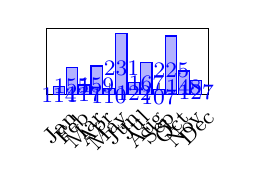
\begin{tikzpicture}
        \begin{axis}[
%            label style={font=\scriptsize},
%            tick label style={font=\scriptsize}
            width = 0.3\textwidth,
            height = 0.2\textwidth,            
            bar width=4pt,
            scaled ticks=false,
            ymajorticks=false,
            ybar stacked,
            enlargelimits=0.09,
            clip=true,
            legend style={at={(0.5,-0.15)},anchor=north,legend columns=-1},          
            xtick=data,
            xticklabel style={rotate=45, font=\footnotesize},
            tick pos=left,
            nodes near coords,
            every node near coord/.append style={font=\footnotesize},
            nodes near coords align={vertical},
            symbolic x coords={Jan, Feb, Mar, Apr, May, Jun, Jul, Aug, Sep, Oct, Nov, Dec},]
            \addplot coordinates {(Jan, 114) (Feb, 155) (Mar, 117) (Apr, 159) (May, 110) (Jun, 231) (Jul, 122) (Aug, 167) (Sep, 107) (Oct, 225) (Nov, 148) (Dec, 127)};
        \end{axis}
      \end{tikzpicture}
    }
    \vspace{-4ex}
    \caption{\label{fig:distribution-rules-per-month}2019 new rules.}
\end{wrapfigure}% <---- don't forget this %

Intuitively, rulesets need to be continuously revised because new
vulnerabilities are discovered and attackers can take advantage of
them. Unfortunately, creating these rules is time-consuming and
error-prone. The language for describing rules is non-trivial (see
Section~\ref{sec:example-suricata-rules}) and testing correctness of a
rule requires data and careful inspection.


%% IT-security companies capitalize on this phenomena and
%% offer rulesets on the
%% market.

This paper proposes \tname{}\footnote{Abbreviation for
  \textbf{Sy}nthesis of Su\textbf{ri}cata R\textbf{u}le\textbf{s}.}, a
technique that uses machine intelligence to automatically synthesize
rules for rule-based \nids. Our goal is to facilitate the creation of
rules and, consequently, help system administrators to harden the
protection of \nids\ to network attacks. \tname{} synthesizes rules to
protect against a given attack from 1) malicious traffic (\ie{},
examples of the attack to protect against), 2) benign traffic, and 3)
trusted rules.

\Fix{
denial-of-service
attack to a server by matching specific conditions about the network
traffic~\cite{understanding-dos}. Relevant properties about the
traffic of interest appear in bold in this rule (see
Section~\ref{sec:suri-metas-coverage}). Deployments of rule-based
\nids\ are restricted to a fixed set of rules defined by the network
system administrator.}\Mar{check...}



%% Note that anomaly-based \nids are evolving pretty quick with the
%% advances in machine learning, but rule-based \nids are still extremely
%% popular.  \tname{} could also leverage existing databases of malicious
%% traffic to synthesize rules.  Regardless of how the negative traffic
%% is produced (out of scope of this paper), those rules can be
%% distributed to rule databases for free.
%%  The
%% core motivation is that 1) attackers are productive in creating new
%% ways to circumvent existing protections and 2) manual creation of
%% rules is tedious and time-consuming.  

\Fix{summarize how the technique works}

\Fix{summarize results} We believe these results provide initial
evidence on the effectiveness of \tname{}.

This paper makes the following contributions.

\section{Network Intrusion Detection Systems (\nids)}
\label{sec:background}

This section presents background used in the next sections.

\subsection{Rule-based and Anomaly-based \nids}

\sloppy \nids{} are typically categorized in two
groups~\cite{kumar2007survey}: rule-based, as briefly described on
Section~\ref{sec:intro}, and anomaly-based \nids. An
\emph{anomaly-based intrusion detector} learns usage behavior from
benign traffic and, based on that, alerts uncommon
behavior~\cite{7579764,kumar2007survey,Mitchell:2014:SID:2597757.2542049,cordy-etal-issta19}. More
precisely, an anomaly-based \nids{} flags an attack when the network
traffic manifests different characteristics compared to those of the
benign traffic. Rule-based \nids{} and anomaly-based \nids{} are
complementary. A rule-based \nids{} focuses on known attacks whereas
anomaly-based \nids{} focuses on unknown potential attacks. Rule-based
\nids\ can miss attacks as rulesets can become obsolete whereas
anomaly-based \nids\ can report false alarms as learning algorithms
that generalize observations from bening traffic are approximate.
This paper focuses on rule-based \nids\ for its tremendous popularity
in industry\Fix{cite or tone down}. Although we used Suricata, the
principles we used are general to any other signature-based
\nids~(\eg{}, Snort~\cite{snort}).


\subsection{Suricata Rules}
\label{sec:example-suricata-rules}

Figure~\ref{fig:pingscan-example} shows an example rule of
Suricata~\cite{suricata}, a popular open-source \nids{} maintained by
the Open Information Security Foundation (OISF)~\cite{oisf}.  A
Suricata rule is divided in three parts---action, header, and rule
options~\cite{suri-rule-format}. The \emph{action} appears as the
first word in the rule description (an \CodeIn{alert}, in this
case). An action denotes the task that needs to be executed if the
rule pattern is satisfied.  In this example, an alert message will be
sent to system administrators if the rule pattern is
satisfied\footnote{Technically, an IPS (Intrusion Prevention System)
  differs from an IDS in the action taken when an intrusion is
  observed. IPS systems block malicous traffic whereas IDS system only
  alert them. However, IDS and IPS do not differ in the approaches
  used to detect the intrusion~\cite{ids-ips}.\Mar{check}}. The
\emph{header} comes after the action in the rule description. It
restricts the information flow covered by the rule. The header of this
rule is \CodeIn{icmp any any -> any any}. It instructs Suricata to
inspect \CodeIn{icmp} traffic flowing from any machine and port to any
machine and port.\MyComment{ The variables \CodeIn{\$HOME\_NET} and
  \CodeIn{\$EXTERNAL\_NET} are configurable.} Finally, \emph{rule
  options} come after the header. It is a semi-colon-separated
sequence of key-value pairs. Rule options serve to document the
analyzed traffic (\eg{}, ``msg'', ``classtype'', and ``sid'') and to
characterize the attack pattern (\eg, ``flags'', ``threshold'', and
``content''). \tname{} produces options of the second kind, which are
\emph{relevant} to capture the attack. For example, the option
\CodeIn{content:<arg>} checks if the argument is present in the
payload of a message.

\vspace{-1ex}
\begin{table}[h!]
  \footnotesize
  \caption{\label{table:rules}Example of non-documentation options of Suricata.}
  \vspace{-2ex}
  \centering
  \begin{tabular}{clp{5.5cm}}
    \toprule
    \multicolumn{1}{c}{\#} & \multicolumn{1}{c}{Name} &  \multicolumn{1}{c}{Description}\\
    \midrule     
    1 & dsize & matches on the size of the packet payload\\
    2 & itype &  matches on a specific ICMP type\\
    3 & icode & matches on a specific ICMP code\\
    4 & icmp\_seq  & checks a ICMP sequence number\\
    5 & icmp\_id & matches on specific ICMP id-values\\
    6 & window & checks the size of the TCP window\\
    7 & flags & matches on TCP flags\\
    8 & fragbits & checks if the fragmentation or reserved bits are set in the IP header\\
    9 & threshold & minimum threshold for a rule before it generates alerts\\
    10 & content & checks if argument is present on the payload\\
    \bottomrule
  \end{tabular}
\end{table}
%\vspace{-1ex}

Table~\ref{table:rules} shows a sample of non-documentation options of
Suricata. Column ``\#'' shows the option number, column ``Name'' shows
the name of the option, and column ``Description'' summarizes
purpose. The option \CodeIn{content} is common in rules to capture
http attacks and http rules are the most common in the Emerging
Threats Open Ruleset~\cite{emerging-threats-open}. The content option
takes a sequence of bytes as argument and checks if that sequence is
present in the payload of the message.  For example, the option
\CodeIn{content:''SELECT''} checks if the string ``SELECT'' is present
in the payload.  Detailed description of the Suricata rules can be
found elsewhere~\cite{suri-rule-format}. It is worth noting that
Suricata supports a total of \totoptions\ distinct options covering
\numproto\ distinct network protocols.


%% A total of 9 of these options
%% are for documentation.\MyComment{For instance, the purpose of rule
%%   option \CodeIn{msg} is to print on the output an informative message
%%   indicating what kind of intrusion has been observed.}
%% Figure~\ref{fig:distribution-rules-protocol} shows the distributions
%% of these options per protocol. The sum of the number of protocol
%% options is higher than \totoptions\ as some options are shared across
%% different protocols. \tname{} does not make distinction among protocols.


%% %\begin{wrapfigure}[14]{r}{0.5\textwidth}
%% \begin{figure}[t!]
%%   \centering
%% %  \vspace{-7ex}
%%   \scalebox{0.85}{
%%     \begin{tikzpicture}
%%       \begin{axis}[
%%           ybar stacked,
%%           enlargelimits=0.15,
%%           legend style={at={(0.5,-0.15)},
%%             anchor=north,legend columns=-1},
%%           %          ylabel={\#rules},
%%           symbolic x coords={dns, ftp, http, icmp, ip, smb, smtp, ssh,
%%           tcp, tls, udp},
%%           xtick=data,
%%           xticklabel style={rotate=45},          
%%           nodes near coords,
%%           every node near coord/.append style={font=\scriptsize},        
%%           nodes near coords align={vertical},
%%         ]
%%         \addplot coordinates {(dns,10) (ftp,11) (http,20) (icmp,18)(ip,16) (smb,13) (smtp,11) (ssh, 10) (tcp, 32) (tls,18) (udp, 18)};
%% %        \legend{relevant, irrelevant}
%%       \end{axis}
%%     \end{tikzpicture}
%%   }
%%   \vspace{-2ex}
%%   \caption{\label{fig:distribution-rules-protocol}Number of relevant
%%     options per protocol supported by Suricata.\Mar{not sure if this
%%       is really helpful.}}
%% %\end{wrapfigure}
%% \end{figure}
  

\subsection{Rules and Packets}
\label{sec:rules-and-packets}

We mentioned above that http rules often used content options, which
associate with the message payload. For non-http rules, options are
often associated with packet fields. Let us consider a rule for an
ICMP attack as example. Figure~\ref{fig:icmp-packet-layout} shows the
layout of an ICMP packet. The packet fields ``Flags'' and ``Time to
Live'', declared in the IP header, are mapped to the \suri\ options
\CodeIn{flagbits} and \CodeIn{ttl}, respectively. Likewise, the fields
``Type'' and ``Code'', declared in the ICMP header, are mapped to the
options \CodeIn{itype} and \CodeIn{icode}, respectively. The values of
the options ``ttl'', ``itype'', and ``icode'' are the same as the
value of the corresponding fields in the ICMP packet. For the field
``Flags'' the value of the corresponding option is encoded in a
bitvector. For example, if the ``Flags'' field stores the value 1010,
the corresponding rule option will be \CodeIn{flagbits:RM}, as each
position of the vector encodes a different character in the
\CodeIn{flagbits} rule option. In summary, the value of several
options can be determined through transformation functions, as those
informally described above. One exception to this is the option
\CodeIn{threshold}, which is typically used in denial-of-service
attacks. That option operates over sequence of messages as opposed to
a single message. Consequently, it is not possible to determine its
values from a single message.

\begin{figure}[t!]
\centering
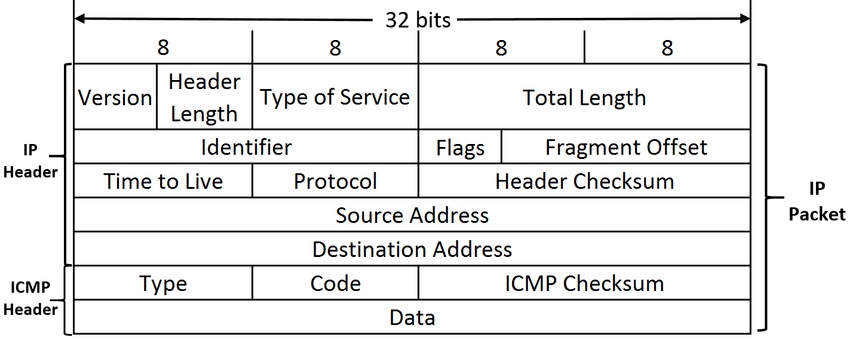
\includegraphics[scale=0.28]{figs/ICMP-packet-structure.png}
\vspace{-2ex}
\caption{Layout of an ICMP packet.}
\label{fig:icmp-packet-layout}
\end{figure}
%\vspace{-2ex}

%% More precisely, to trigger an action on a rule
%% containing that option a \nids\ tool needs to monitor several
%% messages.

%% \Luc{
%%   Os campos Flags e Time to live no header IP são mapeados para as opções fragbits e ttl, respectivamente. Os campos Type e Code no header ICMP são mapeados para as opções itype e icode. \\
%% Os campos, Time to Live, Type e Code recebem diretamente o valor que está no pacote. Por exemplo, se o campo Type no pacote possuir valor 8, na regra ele vai aparecer como itype:8.\\
%% O campo Flags é intepretado como um vetor de bits, onde cada posição representa uma flag. Na regra, o valor do campo Flags é traduzido em caracteres que representam cada flag presente no pacote. Por exemplo: se o campo Flags possuir o valor 1010, na regra aparecerá fragbits:RM, pois os caracteres R e M indicam a presença do quarto e segundo bits.}


\section{Illustrative Example}
\label{sec:suri-metas-coverage}
\label{sec:active-recon}

This section briefly shows how \tname{} synthesizes rules for one
example attack. Active Reconnaissance is typically used as a
preliminary step towards an actual attack. It is a method to collect
information about a computing system to determine potential
vulnerabilities. For example, the Ping Scan attack~\cite{ping-scan}
scans the network for IPs of accessible hosts. An attacker sends
several ICMP Echo requests to a range of IP addresses in the network
and checks which ones respond to these requests. This method enables
an attacker to discover which machines are active in the network.

%\vspace{-1ex}
\begin{figure}[h!]
  \lstinputlisting[language=C,numbers=none,keywords={dsize,itype}]{pingscan.suricata}
  \vspace{-2ex}  
  \caption{Suricata rule for Ping Scan attack.}
  \label{fig:pingscan-example}
\end{figure}
\vspace{-3ex}

Figure~\ref{fig:pingscan-example} shows a Suricata rule that captures
a Ping Scan, as documented in NMAP~\cite{netmap}, a network discovery
and security auditing open-source tool. The essential options to
capture the attack are in bold---the option \CodeIn{dsize: 0}
indicates that the packet has no bytes in the payload and the option
\CodeIn{itype: 8} indicates that the packet to be captured are ICMP
Echo requests.

In the following, we briefly show how \tname{} synthesizes rules for
this attack. In short, \tname{} takes one or more examples of an
attack---in the form of network messages---and produces rules to
capture that attack. Considering the rule for the Ping Scan attack,
whose example was reproduced with NMAP, \tname{} leaves the action of
the corresponding rule constant (as \CodeIn{alert}) and infers the
header by checking the protocol of the input messages. For example, in
this case, \tname{} sets the header to \CodeIn{icmp any any -> any
  any}, indicating that the rule applies to \CodeIn{icmp} messages and
the most general flow description, \ie{}, it instructs the \nids\ to
analyze the icmp traffic flowing from/to any address and port.  The
rationale for this decision is that the choice of these parameters are
domain-specific and subject to change by the system administrator.

The main challenge in synthesizing rules is to discover the set of
rule options (see Table~\ref{table:rules}) that captures the malicious
traffic, but allows the benign traffic to pass. \tname{} proceeds as
follows to synthesize rule options. First, it analyzes the malicious
traffic to extract options expressed in that traffic. Recall from
Section~\ref{sec:rules-and-packets} that some options can be inferred
from packet contents. \tname{} finds the following five options at
this stage: {\scriptsize{\texttt{\textbf{dsize}:0; \textbf{itype:}8;
      \textbf{icode:}0; \textbf{icmp\_id:}23570;
      \textbf{icmp\_seq:}3439;}}}.  By construction, a rule that uses
this set of options captures the malicious traffic. Unfortunately, the
rule above is overspecified. Informally, the rule includes ``too
specific'' characteristics of the malicious traffic and could
potentially result in false negatives. In this case, although the
options \CodeIn{dsize:0} and \CodeIn{itype:8} are present in the set
of inferred options---as the golden rule from
Figure~\ref{fig:pingscan-example} shows---the others are not.

%% \vspace{-2.5ex}
%% \begin{figure}[h]
%%   \lstinputlisting[language=C,numbers=none,frame=none,keywords={dsize,icode,itype,icmp\_id,icmp\_seq}]{pingscan.suricata.synth}
%% \end{figure}
%% \vspace{-2.5ex}
%% \noindent


Second, \tname{} uses the benign traffic to mitigate the overfitting
problem. In this step, \tname{} searches for alternative rules that
preserve the invariant to capture the positive (/malicious) traffic
but not capture the negative benign traffic. It uses the rule obtained
in the previous step as seed to bootstrap the search for alternative
plausible rules, \ie{}, rules that satisfy the aforementioned
invariant. The search is designed to generate rules containing subsets
of the options declared in the seed rule. Considering this example,
\tname{} produces a total of \pingscanplausible{} plausible rules at
the end of the search. This is a smaller number when compared to $2^n$
option combinations, where $n$ is the number of options contained in
the seed rule ($n=5$, in this case). \tname{} is able to prune the
search space and discard many implausible rules. It is worth noting
that the number of plausible rules that \tname\ produces at this step
can be very high for other example attacks (see column ``\#~Plausible
Rules'' on Table~\ref{table:results}).

Finally, \tname{} ranks plausible rules according to heuristics
obtained by analyzing a database of existing rules. The general
intuition is that new rules should share characteristics with existing
human-written rules. For example, one heuristic function used by
\tname{} leverages the popularity of options for ranking.  The score
of a rule $r$, according to that heuristic alone, is proportional to
the popularity of the options declared in
$r$. Figure~\ref{fig:distribution-options} shows the distribution of
options associated with rules from a public
ruleset~\cite{emerging-threats-open} containing
\numrulessuri\ rules. Note that rules with options \CodeIn{content}
and \CodeIn{flow} are the most common. The options \CodeIn{dsize} and
\CodeIn{itype}, the ones associated with the golden rule, appear as
the 6th and 7th most popular, respectively. But, among the options
inferred by \tname{} at the first step, \CodeIn{dsize} and
\CodeIn{itype} are the most popular. At the end of this step, \tname{}
ranks the golden rule second in the list including
\pingscanplausible{} rules. It is worth noting that
\tname\ consistently ranks the golden rule very high in most of the
cases even when the technique produces a large number of plausible
rules (see Table~\ref{table:results}).

To sum up, \tname{} uses the messages that manifest an attack in the
first step to create a potentially overspecified seed rule. Then, it
uses benign traffic in the second step to create a set of plausible
rules from the seed rule. Finally, in the third step, \tname{} uses
existing rules to learn heuristics to rank plausible rules.

\section{Technique}
\label{sec:technique}

\tname{} is a technique to synthesize rules for rule-based
\nids~(\eg{}, Snort~\cite{snort} and Suricata~\cite{suricata}). The
goal is to automatically create rules that capture an attack of
interest.

\vspace{1ex}
\noindent\textbf{Overview.}~\tname\ takes on input one or more
examples of an attack and produces on output a ranked list of
\emph{plausible rules}---\ie{}, rules that isolate the malicious
traffic produced by the attacks from the benign
traffic. Figure~\ref{fig:overview} shows the workflow of \tname{} as a
pipeline of three components, appearing numbered in the figure.
Public data sets of benign
traffic~\cite{tcpreplay,stratosphere-normal} and rules
exist~\cite{emerging-threats-open}. Consequently, a user of \tname{}
only needs to provide examples of attacks on input.

%% To create rules, \tname\ leverages (1)
%% benign and malicious network traffic and (2) rules from public
%% rulesets. 

\begin{figure}[t!]
  \centering
  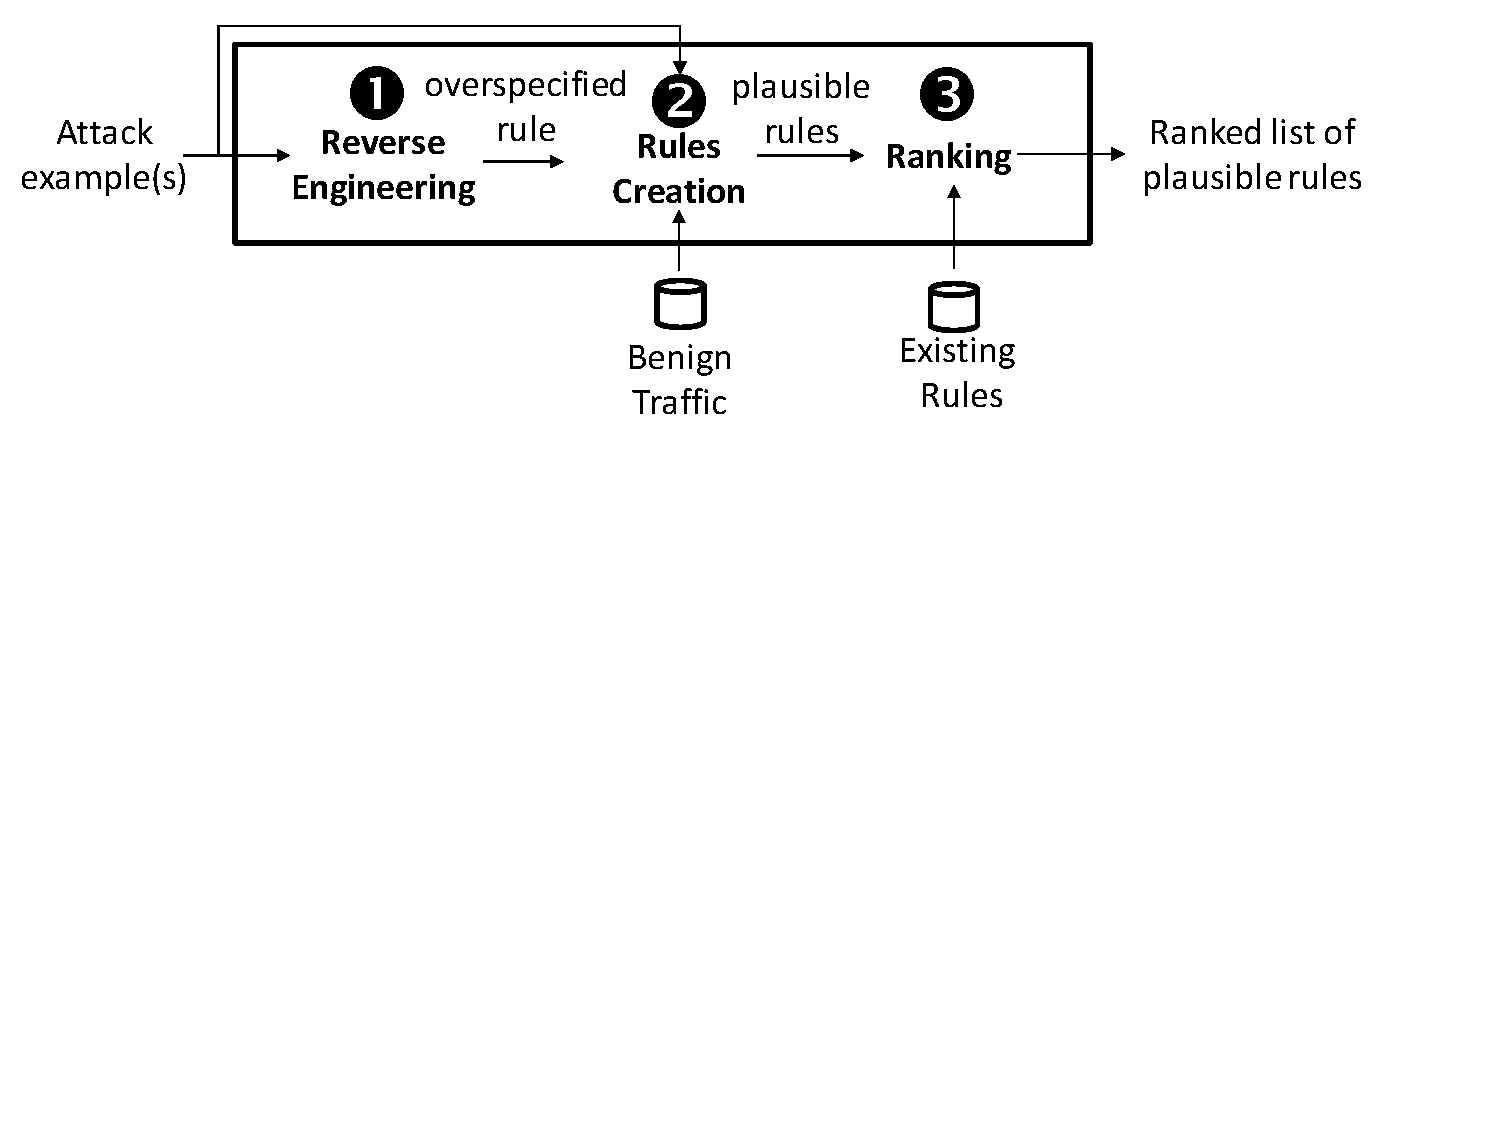
\includegraphics[trim=0 340 50 0,clip,width=0.48\textwidth]{figs/nids-workflow}
  \vspace{-4ex}  
  \caption{The \tname\ workflow.}
  \label{fig:overview}
  \vspace{-3ex}
\end{figure}

\tname\ works as follows. First, it creates a rule that captures the
malicious traffic produced by the examples provided on input. In this
step, \tname\ detects options directly from the input messages (see
Section~\ref{sec:rules-and-packets}). More precisely, it creates a
rule containing options that are guaranteed to be satisfied by the
malicious traffic. Let us refer to that rule as the \emph{seed rule}
and its corresponding set of options as \emph{seed options}. Note
that, as only the malicious traffic is considered in this step, the
seed rule is likely overspecified, \ie{}, it may be more restrictive
than necessary. Consequently, the use of that rule could result in
false negatives. Second, \tname\ generates alternative rules that 1)
weaken the constraints expressed in the seed rule while 2) still
capturing the malicious traffic. Given that every option declared in a
rule needs to be satisfied for a rule to capture an attack, any subset
of the set of seed options, by definition, captures the attack
characterized by the malicious traffic. \tname{} leverages that
observation to search for plausible rules containing a proper subset
of options from the seed options. However, note that that approach
alone could result in false positives as it imposes no limit on the
extent the constraints induced from the rule can be weakened. \tname{}
uses benign traffic for that purpose. More precisely, it searches for
plausible rules derived from the seed rule obtained in the previous
step. Finally, \tname{} uses heuristic functions, obtained from a data
set of existing rules, to rank the generated plausible rules by their
similarity to existing rules. Similarity is used to approximate user's
intent. The following sections detail each component of \tname.

%%  As the generation
%% procedure discards options from the initial rule, the rules \tname{}
%% creates satisfy the property of capturing malicious traffic.



%% The goal of the first
%% component is to produce a rule that captures the negative traffic.
%% First, it initializes the rule with random values. Only options
%% associated with the used protocol are included in the rule
%% representation. Then, \tname\ optimizes the rule options until
%% \suri\ is able to capture the attack associated with the negative
%% traffic.  \tname\ unsuccessfully terminates at this point if it cannot
%% capture the attack. The second component takes as input the rule
%% produced by the first component and tries to minimize that rule. Note
%% that any subset of options would capture the negative traffic---as all
%% options in the rule need to be satisfied for the negative traffic to
%% be captured---but it can also capture positive traffic. This component
%% systematically discards options from the rule encoding until no
%% positive traffic is captured.



\subsection{Step 1: Reverse Engineering}
\label{sec:reverse-engineering}

The goal of the Reverse Engineering step is to extract options from
the malicious traffic produced by the input example attacks. A rule
that contains these options captures the malicious traffic by
construction. \tname\ uses two strategies to extract options: 1)~the
field strategy applies to any protocol and 2)~the payload strategy
applies only to http.  The decision of which strategy to use is based
on the protocol associated with input traffic--the technique uses the
payload strategy if http is detected; otherwise, it uses the field
strategy. We elaborate these strategies in the following.

For the field strategy, \tname{} parses the input messages looking for
options associated with the data in the fields of
messages. Section~\ref{sec:rules-and-packets} shows the correspondence
between packet fields and some of the rule options from \suri\ and
Section~\ref{sec:active-recon} shows a concrete example illustrating a
case of this strategy. We obtained the option-field mapping
manunually, from the \suri\ documentation.

Unfortunately, the relevant data for the option may be at the message
payload; not the fields. By analyzing our data set of rules, we found
that this occurs frequently in http attacks, which are prevalent. For
example, \percHttp\ of the \numrulessuri{} rules from the ruleset we
analyzed~\cite{emerging-threats-open} prescribe defenses against http
attacks. In addition, \percRulesWithContent{} of these rules contain
at least one content option. Figure~\ref{fig:rule-jboss} shows an
example of a rule that captures traffic containing the string
\CodeIn{"/HtmlAdaptor"} in the payload.
Figure~\ref{fig:distribution-contents} shows the distribution of
number of content options per rule for the data set mentioned
above. We limited the number of content options per rule to 10 in the
histogram for space. \MyComment{Rules without \CodeIn{content} options
  are an exception and half of the rules contain at least two
  \CodeIn{content} options.}  To sum up, handling content options for
http is very important.

The content strategy focuses on extracting content options from the
message payload. By inspecting existing rules, we found that these
options refer to sequences of characters separated by typical natural
language delimiters such as $\backslash$t, $\backslash$n,
$\backslash$r, and spaces. To find the values associated with these
options, \tname{} splits the payload in tokens using these delimiters.
Considering the example from Section~\ref{sec:content-example},
\tname{} produced a total of 23 tokens\Mar{@Lucas, isto estah certo?
  Se sim, como isto cai para 5 (pela Tabela 3)}, considered content
option candidates.

It is worth noting that we found that deciding which reverse
engineering strategy to use based on the protocol of the input
(malicious) messages was effective. We used the payload strategy for
http and the field strategy for the other protocols. For flooding
attacks, \tname\ runs the same approach for each message and
identifies common options across all messages. For that case,
\tname\ reports, in addition, a \CodeIn{threshold} option, as
discussed on Section~\ref{sec:rules-and-packets}.  At the end of the
Reverse Engineering step, \tname\ produces a seed rule that captures
the malicious traffic.

%% \Mar{Nao esta muito claro como isto funciona. Rodamos sempre as duas
%%   estrategias (para obter field options e content options)?
%%   (Precisamos dizer se eh possivel ter regras com os dois tipos de
%%   opcoes). Como isto funciona 1) quando uma ataque tem varias
%%   mensagens (e.g., ping scan) e 2) quando temos varios ataques?}

%% \textbf{Implementation.}~
%% , characterized with pcap files~\cite{pcap}, a popular format
%% to describe network packets.

%% \Fix{
%% A avaliação que fazemos aqui pontua um dado content de acordo com
%% quantas vezes o campo em que ele se encontra eh referenciado nas
%% regras. Por exemplo, vamos supor que o tokenizer produziu a opção
%% content: "/HtmlAdaptor". Essa string pertence ao campo "Request
%% URI:". Esse campo pode ser acessado pelo modificador http\_uri. O
%% tokenizer associa o content a esse modificador.
%% }


\subsection{Step 2: Rules Creation}
\label{sec:minimization}

The seed rule produced in the first step satisfies the criterion to
capture the traffic produced by the example attacks. However, that
rule is overconstrained.  It may include options that are irrelevant
to capture the attack and lead to false negatives---the \nids\ may be
unable to capture manifestations of the same attack whose messages do
not exhibit the data satisfying irrelevant options. For example, the
seed rule produced after the Reverse Engineering step on the Ping Scan
example from Section~\ref{sec:active-recon} contains options
\CodeIn{icode:0}, \CodeIn{icmp\_id:23570}, and
\CodeIn{icmp\_seq:3439}, which are irrelevant to capture that attack.

%%  Some options added to the rule
%% during the first step are irrelevant for determining the attack and
%% should be removed to obtain more general rules. 

To address the overffiting issue, \tname{} leverages public data sets
of benign traffic~\cite{tcpreplay} and additional examples of the
attack to guide the search for more general rules. To that end,
\tname{} \emph{minimizes} the rules produced in the previous step,
preserving the invariant of \emph{only} capturing the positive
malicious traffic. We say that a rule is minimal if discarding any
option results in the capture of negative (\ie{}, benign) traffic.
The procedure we propose in this step builds on the observation that
all options from the rule produced in the previous step are satisifed
by the traffic produced by the attack. Consequently, any subset of
these options also captures the attack. The rule creation procedure
iteratively discards options from visited rules---derived from the
seed rule---using the negative traffic to guide the search for minimal
rules.

\algdef{SE}[DOWHILE]{Do}{doWhile}{\algorithmicdo}[1]{\algorithmicwhile\ #1}%
\algnewcommand\algorithmicforeach{\textbf{for each}}
\algdef{S}[FOR]{ForEach}[1]{\algorithmicforeach\ #1\ \algorithmicdo}
\algnewcommand\And{\textbf{and} }%
\setlength{\textfloatsep}{3pt}% Remove \textfloatsep
\begin{algorithm}[t!]
  %\noindent\hspace{-2ex}
  \flushleft{}\textbf{INPUT:} (overconstrained) seed rule $sr$, pcap
  files for bening traffic\\
  ($\mathit{bTr}$), pcap files for mallicious traffic ($\mathit{mTr}$)\\
  %\noindent\hspace{-27.5ex} 
  \textbf{OUTPUT:} Set of minimized rules $\mathcal O$\\
%\vspace{-3ex}
\captionof{algorithm}{Rule creation algorithm}\label{algo1}
\begin{algorithmic}[1]
  \State $\mathcal R \gets \{\mathit{sr}\}$\Comment{initial population of candidate solutions.}\label{line-init}
  \State $\mathcal O \gets \emptyset$
  \Do\label{start-do-while}
      \State $\mathcal R' \gets \emptyset$ \Comment{new iteration. reset.}\label{init-rprime}
      \ForEach {$ro \in \mathcal R $}\Comment{analyze each candidate rule.}\label{start-foreach}
           \For {$i \gets 1$ to $N$}\Comment{mutate each rule $N$ times.}\label{start-for}
               \State $r \gets copy(ro)$\label{copy}
               \State $j\gets \mathit{rand}(0,\mathit{len}(r))$\label{choose-index}
               \State $r[j]\gets 0$\Comment{discard option $j$ in $r$}\label{delete-option}
               \If{$\mathit{isNew(r)} \And\mathit{isPlausible}(r, \mathit{bTr})$} 
                   \State $\mathcal R' \gets \mathcal R' \cup \{r\}$\label{line-progress}
               \EndIf
           \EndFor\label{end-for}
       \EndFor\label{end-foreach}
       \State $\mathcal R \gets \mathcal R'$\Comment{update new generation}\label{define-next-gen}
       \State $\mathcal O \gets \mathcal O \cup \mathcal  R$\Comment{remember all rules}\label{output-accum}
  \doWhile{$\mathcal R\not= \{\}$}\Comment{repeat until reaching a
    fixpoint}\label{end-do-while}\\
  \Return $\mathit{filter(\mathcal O, mTr)}$\label{filtering}
\end{algorithmic}
\end{algorithm}

Algorithm~\ref{algo1} shows the pseudocode for deriving rules from the
seed rule produced at the Reverse Engineering step. The algorithm
takes as input an overconstrained rule $sr$ and pcap files~\cite{pcap}
to reconstruct the benign ($\mathit{bTr}$) and malicious traffic
($\mathit{mTr}$). The algorithm produces on output a set of
alternative rules to $sr$ that captures every instance of the attack
(as per $\mathit{mTr}$), but does not capture any message from the
benign traffic (as per $\mathit{bTr}$).

Line~\ref{line-init} initializes the current population of individuals
(\ie{}, rules) $\mathcal{R}$ with the seed rule $sr$. We encode a rule
as a bitvector where each index in the vector represents one option;
the value assigned at a given position indicates whether or not the
option is present in the rule. One iteration of the outer loop
(lines~\ref{start-do-while}-\ref{end-do-while}) processes the current
population of individuals $\mathcal R$ and creates the next generation
$\mathcal R'$. Line~\ref{init-rprime} initializes the population of
individuals for the next generation. The inner loop
(lines~\ref{start-foreach}--\ref{end-foreach}) iterates through each
candidate rule in $\mathcal R$. The algorithm mutates each of these
rules for $N$ times, discarding one option of the rule each
time. Line~\ref{copy} assigns a copy of the bitvector, encoding
$\mathit{ro}$, to variable $r$. Function $\mathit{len}$ returns the
length of a vector and function $\mathit{rand}$ randomly chooses one
integer value in the range defined by its parameters. So, the
expression $\mathit{rand(0, len(r))}$, appearing at
line~\ref{choose-index}, returns an index of the option in $r$ to
delete at line~\ref{delete-option}. The call to $\mathit{isNew}$
checks if $r$ has not been previously generated in another iteration
whereas the call to $\mathit{isPlausible}$ checks if the rule only
captures positive traffic, \ie{}, it checks that no message present in
$\mathit{bTr}$ is captured by $r$. If $r$ satisfies both criteria, it
is added to $\mathcal R'$, which denotes the next generation of
individuals in the search. After processing every candidate rule in
$\mathcal R$, the next generation of individuals is defined
(line~\ref{define-next-gen}) and the set of discovered rules is
updated (at line~\ref{output-accum}).

The do-while loop terminates when no rule in the current generation of
individuals can be further reduced without violating the invariant
that a candidate solution should only capture positive traffic. This
means that execution of one iteration of the do-while loop has not
reached the statement declared at line~\ref{line-progress}, which adds
one element to the set $\mathcal{R'}$. As $\mathcal{R'}$ is
initialized empty, that set will remain empty at the end of the
execution of the loop from
lines~\ref{start-foreach}-\ref{end-foreach}. The algorithm returns the
rules from $\mathcal O$ that capture \emph{all} example attacks
provided on input (line~\ref{filtering}).

Note that the algorithm produces no rules in the last iteration. Rules
with a single option are produced in the second-to-last iteration. In
other iterations, rules with more than one option are
produced. Conceptually, the search induces a search tree with the seed
rule $sr$ as root, single-option rules as child nodes, and rules with
more options as internal nodes. The edges of the tree denote the
ancestor relation between a pair of rules. It is also worth noting
that the algorithm reports every rule in the tree instead of only
those with one option. The reason is that the traffic used to check
plausibility is limited by definition---reporting only minimal rules
with respect to that traffic could discard the correct rule.

In summary, this algorithm reports many rules that are plausible by
using the benign traffic to reduce the overconstrained rule produced
at the \reveng\ step. In the Raking step (Section~\ref{sec:ranking}),
\tname{} ranks the rules this algorithm reports by their similarity to
existing trusted rules. Intuitively, rules that do not look like those
trusted rules rank low.

\begin{proposition}
  \vspace{-1ex}  
  The rule generation algorithm reports rules that capture only the
  positive traffic.
\end{proposition}
\begin{proof}
  \vspace{-1.5ex} Every rule created during the search captures the
  attack provided as example on step one as every created rule
  contains a proper subset of the options from the original rule and
  all those options are, by definition, satisfied by the traffic
  produced by the original attack. In addition, from the definition of
  function $\mathit{isPlausible}$, reported rules capture \emph{only}
  the positive traffic. If negative traffic is captured, a rule is not
  added to $\mathcal R'$. Consequently, it cannot be an element of
  $\mathcal O$ and reported on the output. Finally, from the
  definition of function $\mathit{filter}$, only the rules in
  $\mathcal O$ that capture all the instances of the attack (\ie{},
  variants) are reported on output.
  \vspace{-1ex}    
\end{proof}

%% \begin{proposition}
%%   The minimization algorithm may not produce minimal rules.
%% \end{proposition}

%% \begin{proof}
%% The output of the minimization algorithm may contain rules that are
%% not minimal given the non-determinism of the algorithm. In principle,
%% it is possible that options that could be discarded are not selected
%% in the loop from lines~\ref{start-for}--\ref{end-for}. However, we
%% found empirically that a small value of $N$ suffices to discard those
%% options from a rule.
%% \end{proof}

%% Public databases of negative traffic with
%% \Fix{thousands} of messages exist  and can be used to
%% increase the accuracy of the minimization.
%\subsection{Limitations}
%\Fix{...}

\textbf{Implementation details.} We implemented function
\emph{isPlausible} by 1)~updating Suricata to only monitor the rule
that is passed as parameter\Mar{isto realmente eh necessario? se sim,
  explique. me pareceu que o que vc. precisa ate aqui jah estaria no
  log do \suri}, 2)~replaying the negative benign traffic (see
Section~\ref{sec:dataset-benign}), and 3)~reading the Suricata logs to
check if any benign message was captured by the rule. \Mar{discuss
  filter function.} It is worth
noting that the benign traffic is stored in \emph{pcap}
files~\cite{pcap} and Suricata can process those files very
efficiently compared to analyzing network messages directly. Instead
of sending traffic to a machine with a deployed server (\eg{}, web
server) that \suri\ would monitor, our setup calls \suri\ directly
through an API. \suri\ is invoked multiple times in the process of
minimizing the rule.  \textbf{Limitations.} It is worth noting that
the performance of \tname{} depends on the quality of inputs. For the
positive malicious traffic, \tname{} only requires one sample (as
input to step one), but can benefit of several samples (see
line~\ref{filtering} of Algorithm~\ref{algo1}). The same applies to
the negative traffic. However, in this case, \tname{} can use a large
variety of public data sets available online (see
Section~\ref{sec:objectanalysis-benign}).

\subsection{Step 3: Ranking}
\label{sec:ranking}

\tname{} uses a composition of heurisitic functions to sort the rules
produced in the previous step. Each of these functions uses a
different criterion to estimate how similar a created rule is to those
from public rulesets~\cite{emerging-threats-open}. The intuition is
that rules that look more similar to existing trusted rules are more
likely to be useful. The aggregated score of a rule is the weighted
average across the values produced by each heuristic function. The
codomain of each function ranges on the 0-1 interval. Hence, the score
of a rule also ranges on the 0-1 interval. We describe in the
following each of these heuristic functions.

%% \Luc{atualmente eh uma
%%   média simples e não ponderada ja q as funções tem o mesmo
%%   peso. conversamos na ultima reuniao sobre testar diferentes pesos
%%   para cada função, mas n sei quão prioritário eh isso comparado as
%%   outras atividades que definimos.} $\sum{f_i}/|f_i|$.

%% Note that there are 11 rules with no
%% options. These rules only use the header to signal a traffic as
%% malicious. Also note that most rules have 2 to 6 options. 

\subsubsection{\label{sec:popularity-options}Popularity of options.}
One heuristic function that \tname{} uses to measure similarity
between a synthesized rule and a human-created rule is the popularity
of the options used in those rules. According to this heuristic, rules
containing popular options score higher compared to those containing
unpopular rules. Figure~\ref{fig:distribution-options} shows the
histogram of rule options for the ruleset we
used~\cite{emerging-threats-open}. The x-axis shows the options used
in rules (the 10 most common) and the y-axis shows the number of rules
using the corresponding option. Note that the options
\CodeIn{content}, \CodeIn{flow}, and \CodeIn{prce} are very
popular. \tname\ uses the following formula to compute the
contribution of option popularity to the score of a rule $r$:

{\small
\vspace{-2ex}
\[\sum_{i=1}^{N}\frac{\mathit{option\_frequency[option_i]}}{\mathit{max(option\_frequency)}}/N\]
\vspace{-2ex}
}

\noindent
The term $\mathit{option_i}$ denotes the $i$th option in the bitvector
encoding $r$. The term $\mathit{option\_frequency}$ encodes the
distribution of option popularity as a dictionary mapping
numbers---indicating popularity---to corresponding
options. Consequently, the term $\mathit{option\_frequency[option_i]}$
denotes the number of rules, from our dataset, containing
$\mathit{option\_i}$. The term $\mathit{max(option\_frequency)}$
refers to the maximum number of rules for any dictionary entry (to
normalize the measurement in the 0-1 range), and $N$ is the number of
options in $r$. To illustrate, the contribution of this function to
the score of a rule would be $0.26$ ($=(10181+3049)/(2*25699)$) for a
rule with options \CodeIn{prce} and \CodeIn{flowbits} and $0.01$
($=(155+108)/(2*25699)$) for a rule with options \CodeIn{itype} and
\CodeIn{icode}.

%% \Gui{A quinta heuristica que utilizamos
%%   considera a popularidade das opcoes. Primeiro pegamos a quantidade
%%   de vezes que uma opcao eh utilizada (sem considerar repeticoes numa
%%   unica regra). Dividimos o valor encontrado para cada opcao pelo
%%   maior valor encontrado, encontrando sempre valores de no maximo
%%   1. Entao na regra nos somamos os valores de cada opcao, dividido
%%   pelo numero de opcoes, chegando a um numero de no maximo 1, que
%%   representa a popularidade das opcoes na regra.}

%% \subsubsection{Size of a rule}
%% \label{sec:heuristic-size-of-rule}
%% \tname{} values rules in that size range higher compared to
%% other sizes.

%% We calculate the contribution of size of a given rule
%% $r$ with the  $\mathit{rules\_per\_size}[\mathit{len(r)}]/\mathit{max(rules\_per\_size)}$, where $\mathit{len(r)}$ denotes the number of options of a rule $r$,
%% $\mathit{rules\_per\_size}$ encodes the distribution of sizes as a
%% dictionary mapping sizes to number of associated rules, and
%% $\mathit{max(rules\_per\_size)}$ returns the maximum number of rules
%% for any dictionary entry as to normalize the measurement in the 0-1
%% range. 
%% Consequently, the contribution of size is proportional to its
%% popularity. The contribution of this heuristic would be 0.684
%% (=3,662/5,353) to a rule with three options and 0.028 (=154/5,353) to
%% a rule with nine options.




%% \vspace{-2ex}
%% \[\]
%% \vspace{-2ex}
%\noindent

%% \Luc{Se for preciso temos numeros para fundamentar isso
%%   melhor, sao cerca de 70K contents nas 28K regras do
%%   data set}\Mar{sim, isto ajuda, porem mais importante eh saber quantas
%%   (\%) das 28K regras tem contents.} \Luc{92\%}

\pgfplotsset{width=6cm,compat=1.8}
\pgfplotsset{every tick label/.append style={font=\tiny}}

%%   \begin{subfigure}{.25\textwidth}
%%     \centering
%%     \scalebox{0.8}{
%%       \begin{tikzpicture}
%%         \begin{axis}[
%%           bar width=4pt,
%%           scaled ticks=true,
%%           ymajorticks=false,
%%           ybar stacked,
%%           enlargelimits=0.08,
%% %          enlargelimits=false,
%% %          axis equal,
%%           clip=false,
%%           legend style={at={(0.5,-0.15)},anchor=north,legend columns=-1},          
%%           xtick=data,
%% %          xticklabel style={rotate=45},          
%%           nodes near coords,
%%           every node near coord/.append style={font=\scriptsize},
%%           xticklabel style={font=\footnotesize},          
%%           nodes near coords align={vertical},
%%           symbolic x coords={0, 1, 2, 3, 4, 5, 6, 7, 8, 9, 10},
%%           ]
%%           \addplot coordinates {(0,11) (1,1301) (2,4910) (3,3662) (4,3250) (5,5353) (6,2911) (7, 1337) (8, 1246) (9,763) (10, 495)};
%%         \end{axis}
%%       \end{tikzpicture}
%%     }
%%     \vspace{-1ex}
%%     \caption{\label{fig:distribution-rule-size}Rule sizes.}
%%   \end{subfigure}%

\begin{figure}[t!]
  \centering
\begin{subfigure}{.25\textwidth}
  \centering
  \scalebox{0.8}{  
    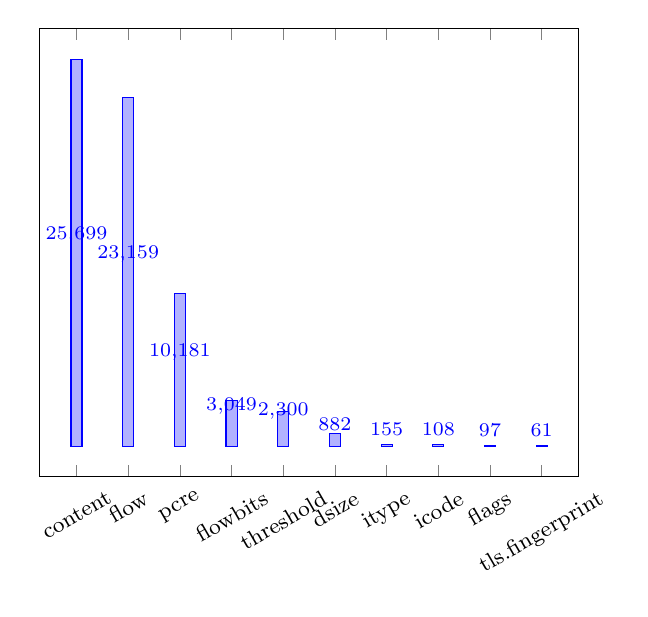
\begin{tikzpicture}
      \begin{axis}[
          bar width=4pt,
          scaled ticks=true,
          ymajorticks=false,
          ybar stacked,
          enlargelimits=0.08,
%          enlargelimits=false,
%          axis equal,
          clip=false,
          legend style={at={(0.5,-0.15)},anchor=north,legend columns=-1},          
          xtick=data,
          xticklabel style={rotate=30},
          nodes near coords,
          every node near coord/.append style={font=\scriptsize},
          xticklabel style={font=\footnotesize},          
          nodes near coords align={vertical},
          symbolic x coords={content, flow, pcre, flowbits, threshold, dsize, itype, icode, flags, tls.fingerprint},          
        ]
        \addplot coordinates {(content,25699) (flow,23159) (pcre,10181) (flowbits,3049) (threshold,2300) (dsize,882) (itype,155) (icode, 108) (flags, 97) (tls.fingerprint, 61)};
      \end{axis}
    \end{tikzpicture}
  }
  \vspace{-5ex}
  \hspace{4ex}
  \caption{\label{fig:distribution-options}Option popularity.}
%  \vspace{-1ex}    
\end{subfigure}%  
  \begin{subfigure}{.25\textwidth}
    \centering
    \scalebox{0.8}{  
      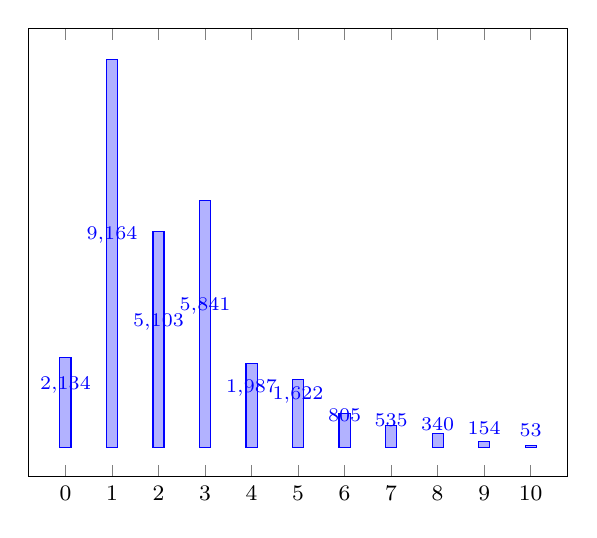
\begin{tikzpicture}
        \begin{axis}[
bar width=4pt,
          scaled ticks=true,
          ymajorticks=false,
          ybar stacked,
          enlargelimits=0.08,
%          enlargelimits=false,
%          axis equal,
          clip=false,
          legend style={at={(0.5,-0.15)},anchor=north,legend columns=-1},          
          xtick=data,
%          xticklabel style={rotate=45},          
          nodes near coords,
          every node near coord/.append style={font=\scriptsize},
          xticklabel style={font=\footnotesize},          
          nodes near coords align={vertical},
          symbolic x coords={0, 1, 2, 3, 4, 5, 6, 7, 8, 9, 10},
          ]
          \addplot coordinates {(0,2134) (1,9164) (2,5103) (3,5841) (4,1987) (5,1622) (6,805) (7, 535) (8, 340) (9,154) (10, 53)};
        \end{axis}
      \end{tikzpicture}
    }
    \vspace{-1ex}
    \caption{\label{fig:distribution-contents}Number of content options.}
  \end{subfigure}% <---- don't forget this %
  \\
\begin{subfigure}{.25\textwidth}
  \centering
  \scalebox{0.8}{  
    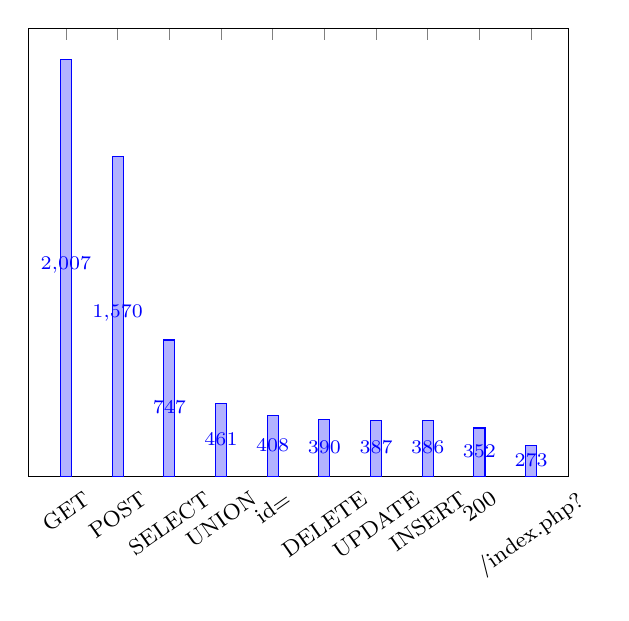
\begin{tikzpicture}
      \begin{axis}[
          bar width=4pt,
          scaled ticks=true,
          ymajorticks=false,
          ybar stacked,
          enlargelimits=0.08,
%          enlargelimits=false,
%          axis equal,
          clip=false,
          legend style={at={(0.5,-0.15)},anchor=north,legend columns=-1},          
          xtick=data,
          xticklabel style={rotate=35},          
          nodes near coords,
          every node near coord/.append style={font=\scriptsize},
          xticklabel style={font=\footnotesize},          
          nodes near coords align={vertical},
          symbolic x coords={GET, POST, SELECT, UNION, id=, DELETE, UPDATE, INSERT, 200, /index.php?},          
        ]
        \addplot coordinates {(GET,2007) (POST,1570) (SELECT,747) (UNION,461) (id=,408) (DELETE,390) (UPDATE,387) (INSERT, 386) (200, 352) (/index.php?, 273)};
      \end{axis}
    \end{tikzpicture}
  }
  \vspace{-2ex}  
  \caption{\label{fig:distribution-strings}Strings used in content options.}
\end{subfigure}%
\begin{subfigure}{.25\textwidth}
  \centering
  \scalebox{0.8}{
    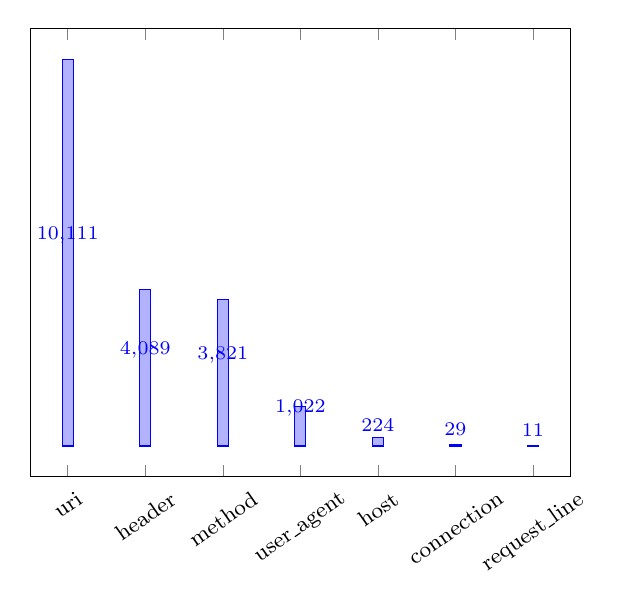
\begin{tikzpicture}
      \begin{axis}[
          bar width=4pt,
          scaled ticks=true,
          ymajorticks=false,
          ybar stacked,
          enlargelimits=0.08,
%          enlargelimits=false,
%          axis equal,
          clip=false,
          legend style={at={(0.5,-0.15)},anchor=north,legend columns=-1},          
          xtick=data,
          xticklabel style={rotate=35},          
          nodes near coords,
          every node near coord/.append style={font=\scriptsize},
          xticklabel style={font=\footnotesize},          
          nodes near coords align={vertical},
          symbolic x coords={uri, header, method, user\_agent, host, connection, request\_line},          
        ]
        \addplot coordinates {(uri,10111) (method,3821) (user\_agent,1022) (header,4089) (host,224) (connection,29) (request\_line,11)};
      \end{axis}
    \end{tikzpicture}
  }
  \vspace{-2ex}
  \caption{\label{fig:distribution-content_modifiers}Http content modifiers.}
\end{subfigure}%
\vspace{-1ex}
\caption{Distributions.}
\end{figure}



\subsubsection{Number of content options.} We observed
that \percContentOptions\ of the rules from the ruleset we analyzed
contain content options, but the distribution of those contents per
rule is not uniform. Figure~\ref{fig:distribution-contents} shows the
distribution of number of contents in a rule. Results indicate nearly
73\% of the rules from our ruleset contain one to three content
options. Hence, we found that that information could help
\tname\ discriminate useful rules. \tname{} computes the contribution
of the number of content options to the score of a rule $r$ with the
fraction
$\frac{\mathit{rules\_per\_number\_of\_contents[len(r)]}}{\mathit{max(rules\_per\_number\_of\_contents)}}$,
where $\mathit{len(r)}$ denotes the number of content options in $r$
and $\mathit{rules\_per\_number\_of\_contents}$ denotes the
distribution of number of contents (encoded with a dictionary as in
the function described on
Section~\ref{sec:popularity-options}). Consequently the term
$\mathit{rules\_per\_number\_of\_contents[len(r)]}$ corresponds to the
number of rules in the ruleset with the same number of contents as
$r$. The denominator of the fraction normalizes the contribution in
the 0-1 range. To illustrate, the contribution of this heuristic
function to the score a rule would be $.64$ $(=5841/9164)$ to a rule
with 3 content options and $.18$ $(=1622/9164)$ to a rule with 5
content options.

%% \noindent
%% The only difference of this formula compared to the one defined on
%% Section~\ref{sec:heuristic-size-of-rule} is the distribution used. The
%% distribution is given by the term
%% $\mathit{rules\_per\_number\_of\_contents}$ denoting a dictionary of
%% number of content options to number of rules that contain that number
%% of content options.


\subsubsection{Popularity of content strings.} 
This heuristic leverages content rarity to discriminate rules---it
weighs higher (respectively, lower) rules that use popular
(respectively, unpopular) strings in content options. The score of a
rule $r$ on this function is given by the arithmetic mean of the
popularity scores of each string used in contents in $r$. More
precisely, the contribution of content rarity is given by the
following formula:

{\small
\vspace{-1.5ex}
\[\sum_{i=1}^{N}\frac{\mathit{content\_frequency[content_i]}}{\mathit{max(content\_frequency)}}/N\]
\vspace{-0.5ex}
}
\noindent
, where $\mathit{content_i}$ denotes the $i$th content in a given
rule, the term $\mathit{content\_frequency[\mathit{content_i}]}$
denotes the frequency of the string used in the $i$th content, the
term $\mathit{max(content\_frequency)}$ denotes the maximum frequency
observed across all strings appearing as content parameters, and $N$
is the number of content options in a given
rule. Figure~\ref{fig:distribution-strings} shows the distribution of
the ten most popular strings in our ruleset. To illustrate, let us
consider a rule with whose content options use the strings ``GET'' and
``ID'', respectively. The contribution of that rule for the
computation of similarity score would be 0.601 (=(1+.203)/2). The
relatively high weight reflects the fact that ``GET'' and ``ID'' are
popular content strings.

\subsubsection{Popularity of http content modifiers.} As previously
mentioned, \percRulesWithContent\ of \suri\ rules involve content
options. Furthermore, nearly half of the rules that use content
options use content modifiers to qualify the search. Http modifiers
typically serve to specify parts of the message payloads that the
input string should be matched against. For example, the modifier
\CodeIn{http\_header} in the option \CodeIn{content: ``keep-alive'';
  http\_header} indicates that the string ``keep-alive'' should be
present in the header of the http message\footnote{A keep-alive
  connection attribute indicates that a single tcp connection should
  remain open for multiple http requests/responses.}. Note that, in
this case, the content modifier refers to a field of an http message,
which appears in the payload of a tcp message, which is the target of
the option \CodeIn{content}. Figure~\ref{fig:http-header-example}
illustrates possible content options used to match against certain
strings that appear in an http message. A check mark (respectively,
cross) indicates a match (respectively, no match).

\begin{figure}[t!]
\centering
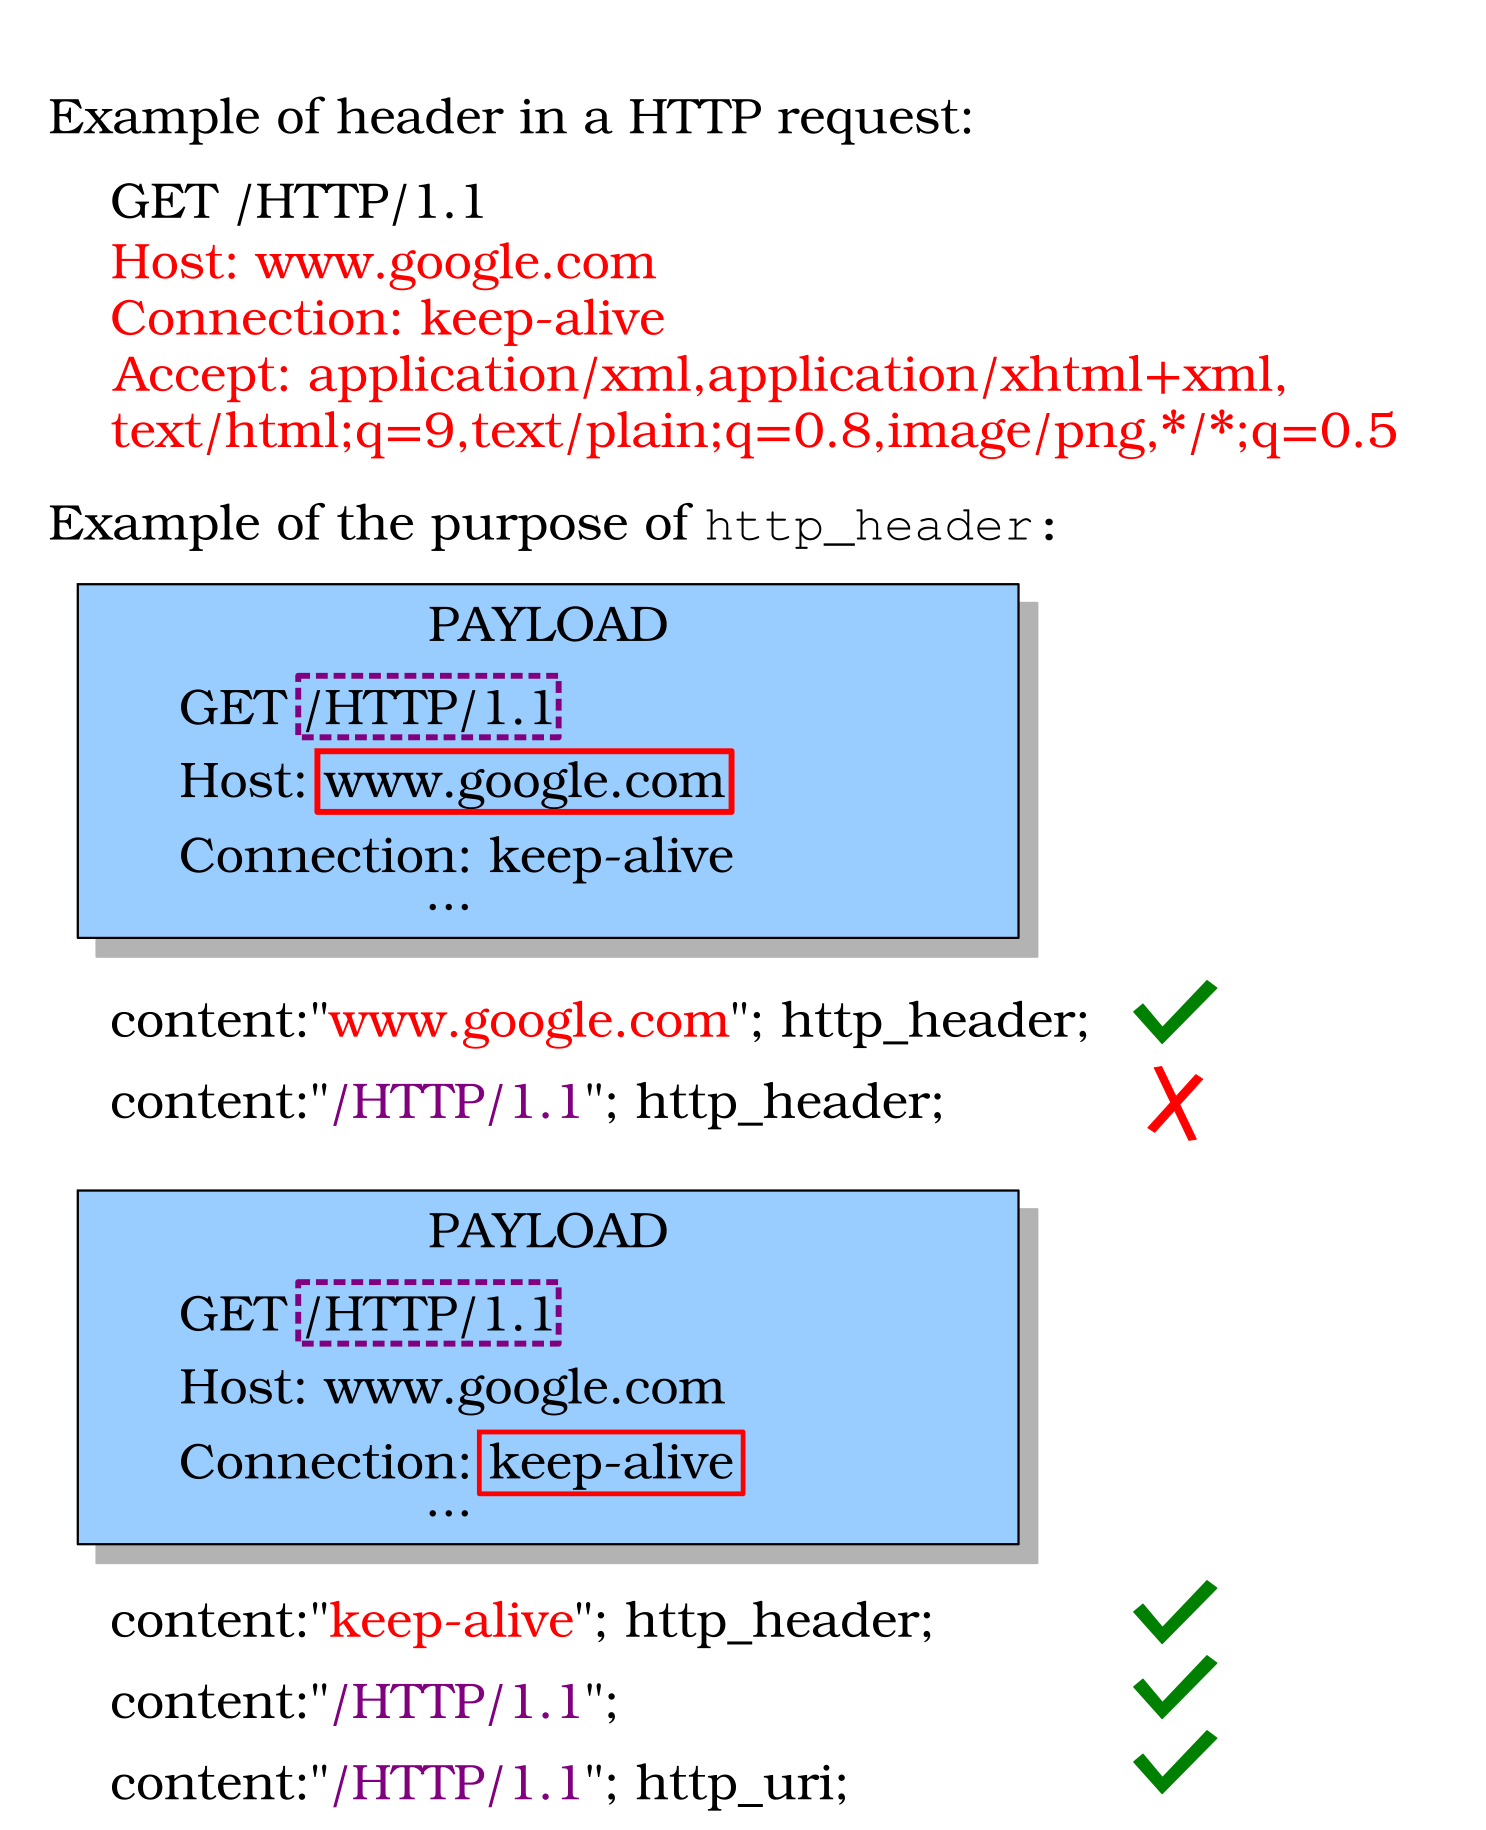
\includegraphics[scale=0.5]{figs/http_header-example.png}
\vspace{-2ex}
\caption{Content modifiers.}
\label{fig:http-header-example}
\end{figure}

\tname\ builds on the observation that the strings commonly accessed
at positions associated with content modifiers (\eg{}, host,
connection) are more common. For example, historical data indicates
that content options that use the modifier \CodeIn{connection} are
much less likely than content options that use the modifier
\CodeIn{uri}. Figure~\ref{fig:distribution-content_modifiers} shows
the histogram of content modifiers for http. (We removed the prefix
\CodeIn{http} on the modifier for space.) Although content modifiers
are applicable to rules of any protocol supported by Suricata,
currently, \tname\ only supports this features for tcp and http; these
rules comprise $\sim$80\% of the rules of our data set. We compute the
heuristic function for content modifiers with the following formula:

\[\frac{\sum_{i=1}^{N}g(i)}{N},~g(i)=\frac{\sum_{j=1}^{M_i}\frac{\mathit{modifier\_frequency[modifier_{ij}}]}{\mathit{max(modifier\_frequency)}}}{M_i}\]

\noindent
, where $g(i)$ is the contribution of content option $i$ to the score,
$N$ is the number of contents options present in a rule,
$\mathit{modifier\_frequency[modifier_{ij}}]$ denotes the popularity
of a modifier $j$ to content option $i$,
$\mathit{max(modifier\_frequency)}$ refers to the modifier with
maximum popularity (for normalization), and $M_i$ is the number of
content modifiers that could access the string associated with content
$i$.
    
To illustrate, consider a rule containing the option
\CodeIn{content:``/HtmlAdaptor''} (see Section~\ref{sec:jboss}). The
contribution of this option---\ie{}, the value of $\mathit{g(i)}$---to
the score of the rule is $0.5$ (=$\frac{10,111+11}{10,111*2}$). The
value of $M_i$, in this case, is 2 as the string ``/HtmlAdaptor''
could be accessed through the modifiers \CodeIn{uri} and
\CodeIn{request\_line}. The reason is that \tname\ identifies that
that string appears in the field \CodeIn{Request URI} (of an http
message from the malicous traffic) and that field is accessible
through these two modifiers. The relatively high heuristic value
reflects the fact that the string could be accessed by two popular
content modifiers.  As another example, consider the option
\CodeIn{content: ``keep-alive''}. In this case, either the modifier
\CodeIn{header} or the modifier \CodeIn{connection} could be used to
locate the string ``keep-alive'', stored in the field
\CodeIn{Connection} from an http message (see
Figure~\ref{fig:http-header-example}). Consequently the contribution
of this heuristic function to the corresponding rule would be $0.2$
(=$\frac{4089+29}{10111*2}$), in this case. Assuming that a rule uses
the two content options mentioned aboved, the aggregated contribution
of this heuristic function to the rule would be 0.35 (=(0.2+0.5)/2).

\subsubsection{Weight Optimization}
\label{sec:weight-optimization}
We optimized the weights of these heuristic functions as follows. We
ran \tname{} using different combinations of weights on a sample of
attacks and chose the combination that offered the best overall
performance, which we computed with the sum of the rankings of the
golden rule on each attack. The weight combination that led to the
smaller sum of positions (of the golden rule) in the rakings was
considered the best choice. We considered \emph{all} combinations of
the following weights 0, 0.25, 0.5, 0.75, and 1. Given that we have
four different functions and five possible weight values, we needed to
run \tname{} on the sample of attacks for 625 (=$5^4$) times. In the
end of the process, the weight combination $\langle{}x,y,z,w\rangle$
was the best we found. \Mar{$\leftarrow$indique aqui quais foram os
  pesos que a gente usar para cada funcao.} Although empirical results
showed that this strategy results in good performance, we remain to
evaluate other optimization strategies, such as evolutionary
alternatives as AVM~\cite{10.1109/32.57624}, to find better weights.
 
%\Gui{Fizemos um teste para encontrar melhores pesos para cada ataque. Calculamos o fitness de cada regra atribuindo diferentes pesos para cada função heurística. Os valores atribuídos foram 0, 0.25, 0.5, 0.75 e 1. Depois de calculado, ordenamos todas as listas criadas e pegamos a posição da Golden Rule. As melhores combinações de pesos (que conseguiram melhor posição da golden rule) estão na tabela 4, onde na coluna "Weights", há quatro números separados por vírgula, cada um deles representando o peso de uma função (na ordem que é representado no paper. O total de regras criadas é igual ao da Tabela 3.}


\setlength{\tabcolsep}{5pt}
\begin{table*}[t!]
  \small
  \caption{\label{table:attacks}List of attacks. Non-http attacks
    appear at the top; http attacks appear at the bottom.}
  \centering
  \begin{tabular}{llllp{8cm}}
    \toprule
    \multicolumn{1}{c}{Name} &
    \multicolumn{1}{c}{Source} &
    \multicolumn{1}{c}{Type} &
    \multicolumn{1}{c}{Protocol} &
    \multicolumn{1}{c}{Groud Truth (relevant/checked options)} \\
    \midrule
    Black Nurse & \cite{pcap-attacks} & DoS & ICMP & \textbf{icode}:3; \textbf{itype}:3; \textbf{threshold}: type both, track by\_dst, count 250, seconds 1;\\    
    Ping Scan & \cite{netmap} & AREC & ICMP & \textbf{dsize}:0; \textbf{itype}:8; \\
    SYN Flood & \cite{hping3} & DoS & TCP & \textbf{flags}: S,12;
    \textbf{threshold}: type both, track by\_dst, count 5000, seconds 5;\\
    UDP Teardrop & \Fix{WireShark} & DoS & UDP & \textbf{fragbits}:M; \textbf{id}:124; \\
    %%UDP Flood & MazeBolt & DoS & UDP & \textbf{fragbits}:M; \textbf{threshold}: type both, track by\_dst, count 5000, seconds 5; \\
    \midrule
    %%Apache Struts 2 & \cite{wrccdc} & RCE & HTTP & \textbf{content}:"POST"; http\_method; \textbf{content}:"java.lang.ProcessBuilder"; nocase; http\_client\_body; fast\_pattern; \textbf{content}:"/struts2-rest-showcase/orders/3"; http\_uri; \\    
    ColdFusion \MyComment{PESC} & \cite{nikto} & PESC & HTTP \MyComment{& Privilege Escalation} & \textbf{content}:"GET"; http\_method; nocase; \textbf{content}:"/CFIDE/administrator"; http\_uri; nocase; \\
    iisadmin access\MyComment{web-application-attack} & \cite{nikto} & RCE & HTTP \MyComment{& Adicionar} & \textbf{content}:"/iisadmin"; nocase; http\_uri; \\
    JBoss JMX\MyComment{ Console Beanshell Exploit} & \cite{nikto} & RCE & HTTP \MyComment{& Remote Code Execution} & \textbf{content}:"/HtmlAdaptor"; nocase; http\_uri; \textbf{content}:"action=inspect"; nocase; http\_uri; \textbf{content}:"bean"; nocase; http\_uri; \textbf{content}:"name="; http\_uri; \\
    Script tag in URI\MyComment{Possible Cross Site Scripting Attempt} & \cite{nikto} & RCE & HTTP \MyComment{& Adicionar} & \textbf{content}:"</script>"; nocase; http\_uri; \\
    WeBid LFI \MyComment{Local File Inclusion} & \cite{nikto} & LFI & HTTP & \textbf{content}:"GET "; depth:4; \textbf{content}:"/cron.php?"; http\_uri; nocase; \textbf{content}:"include\_path="; http\_uri; nocase; \textbf{content}:"../"; \\
    %%WordPress Login & \cite{wrccdc} & PVE & HTTP & \textbf{content}:"log="; http\_client\_body; \textbf{content}:"\&pwd="; http\_client\_body; \textbf{content}:"\&wp-submit="; http\_client\_body; \\
    .htaccess access\MyComment{attempted-recon} & \cite{nikto} & AREC & HTTP \MyComment{& Adicionar} & \textbf{content}:".htaccess"; nocase; http\_uri; \\
    .idq access\MyComment{EXPLOIT ISAPI} & \cite{nikto} & RCE & HTTP \MyComment{& Adicionar} & \textbf{content}:".idq"; nocase; http\_uri; \\
    /system32/ in URI\MyComment{Possible Protected Directory Access Attempt} & \cite{nikto} & AREC & HTTP \MyComment{& Adicionar} & \textbf{content}:"/system32/"; nocase; http\_uri; \\
    Basebuilder LFI & \cite{nikto} & LFI & HTTP & \textbf{content}:"GET"; http\_method; \textbf{content}:"/main.inc.php?"; nocase; http\_uri; \textbf{content}:"mj\_config[src\_path]="; nocase; http\_uri; \\
    Tomcat server snoop access & \cite{nikto} & AREC & HTTP & \textbf{content}:"/jsp/snp/"; http\_uri; \textbf{content}:".snp"; http\_uri;\\  
    \bottomrule
  \end{tabular}
\end{table*}


\section{Evaluation}

This section reports on the evaluation of \tname{}.


\newcommand{\textRQone}{How well \tname\ ranks the golden rule?}
\vspace{0.2cm}
\begin{itemize}[leftmargin=*,label={}]
\item{\textbf{RQ1.}} \textRQone
\end{itemize}

\noindent
\textbf{Rationale.}~The golden rule is a trusted human-written
\nids\ rule that we obtained from credible sources. \tname\ generates
several rules that satisfy the invariant to only capture the malicious
traffic, but the amount of data we used to evaluate that property,
albeit large, is limited. Assessing the quality of each rule
\tname\ produces (\ie{}, fitness to the attack) requires domain
knowledge and much effort. The position of the golden rule at the
ranking produced by \tname\ is a proxy measure to the effort of a
system administrator in finding the rule that fits the purpose.


\newcommand{\textRQtwo}{How important are the heuristic functions
  to \tname's performance?}
\vspace{0.2cm}
\begin{itemize}[leftmargin=*,label={}]
\item{\textbf{RQ2.}} \textRQtwo\
\end{itemize}

\noindent
\textbf{Rationale.}~We proposed a variety of heuristic functions to
rank the plausible rules that \tname\ created during minimization (as
per step 2 in the workflow). Recall that these functions are based on
the data from a public ruleset~\cite{emerging-threats-open} (see
Section~\ref{sec:ranking}). It is therefore important to understand
the extent to which each function contributes to the overall
performance of the technique.

\newcommand{\textRQthree}{How sensitive \tname\ is to the amount of
  positive examples?}
\vspace{0.2cm}
\begin{itemize}[leftmargin=*,label={}]
\item{\textbf{RQ3.}} \textRQthree\
\end{itemize}

\noindent
\textbf{Rationale.}~\tname\ uses both positive and negative examples
to generate rules. This question investigates how sensible the
technique is to the selection of these inputs.
\noindent
\vspace{1ex}

The following sections describe the objects we used to evaluate the
technique (Section~\ref{sec:dataset-benign}), answer the posed
research questions (sections~\ref{sec:answer-rqone},
and~\ref{sec:answer-rqtwo}, and~\ref{sec:answer-rqthree}), and
discuss threats to the validity of the
experiments~(Section~\ref{sec:threats}).


\setlength{\tabcolsep}{2pt}
\begin{table}[h!]
  \small
  \caption{\label{table:results}Results.}
  \vspace{-2ex}
  \centering
  \begin{tabular}{lrrrr}
    \toprule
    \multicolumn{1}{c}{\multirow{2}{*}{Name}} &
    \multicolumn{1}{c}{\multirow{2}{*}{\# Vars.}} &
    \#~Option Cand. &
    \#~Plausible Rules &    
    \multicolumn{1}{c}{Rank} \\

     &
    \multicolumn{1}{c}{} &
    \multicolumn{1}{c}{(step 1)} &
    \multicolumn{1}{c}{(step 2)} &    
    \multicolumn{1}{c}{(step 3)} \\

    \midrule
    Black Nurse & 1 & 4 & 9 & 2 \\    
    Ping Scan & 6 & 5 & 9 & 2 \\
    SYN Flood & 4 & 2 & 2 & 2 \\
    UDP Teardrop & 1 & 4 & 8 & 4 \\
    %%UDP Flood & - & - & - & - \\
    \midrule
    %%Apache Struts 2 & 2 & 65 & - & - \\
    ColdFusion & 7 & 19 & 34 & 3\\
    iisadmin access & 3 & 17 & 408 & 1 \\        
    JBoss JMX & 5 & 23 & 228 & 45 \\
    Script tag in URI & 23 & 22 & 786 & 1 \\
    WeBid LFI & 1 & 23 & 11100 & 10\\    
    %%Wordpress Login & 8 & 59 & - & - \\
    .htaccess access & 5 & 17 & 984 & 2\\
    .idq access & 14 & 19 & 511 & 2 \\
    /system32/ in URI & 4 & 20 & 1,913 & 4 \\
    Basebuilder LFI & 1 & 22 & 18133 & 34 \\
    Tomcat Snoop Access & 1 & 24 & 29830 & 32 \\
    \bottomrule
  \end{tabular}
\end{table}

%%\begin{table}[h!]
%%  \small
%%  \caption{\label{table:weight}Weight Combinations.}
%%  \centering
%%  \begin{tabular}{lrrp{15cm}}
%%    \toprule
%%    \multicolumn{1}{c}{Name} &
%%    \multicolumn{1}{c}{Weights} &
%%    \multicolumn{1}{c}{Rank} \\
%%    \midrule
%%    Ping Scan & - & - \\
%%    SYN Flood & - & - \\
%%    JBoss JMX & 1,0,1,1 & 107 \\
%%    WetedhhtedBid & - & - \\    
%%    ColdFusion & 0,1,1,1 & 7 \\
%%    .htaccess access & 0,1,1,1 & 11 \\
%%    .idq access & 0,1,1,1 & 7 \\
%%    iisadmin access & 0,1,1,1 & 2 \\
%%    /system32/ in URI & 0,1,1,1 & 11 \\
%%    Script tag in URI & 0,1,1,1 & 9 \\
%%    \bottomrule
%%  \end{tabular}
%%\end{table}
%%

\newcommand{\numNonContentAttacks}{5}
\newcommand{\numContentAttacks}{10}

\subsection{Objects of Analysis}
\label{sec:dataset-benign}
\label{attack-reproduction}

This section describes the objects used in \tname{}'s evaluation.

\vspace{1ex}
\subsubsection{Attacks.}~Table~\ref{table:attacks} shows the selection
of attacks we analyzed.  Non-http attacks are listed at the top of the
table whereas http attacks are listed at the bottom. Recall from
Section~\ref{sec:reverse-engineering} that (1) http attacks are
prevalent, (2) most http attacks use only content options, and (3)
most non-http attacks only use field options. We selected from various
sources \numNonContentAttacks\ non-http attacks and
\numContentAttacks\ http attacks. The higher number of http attacks
reflects their popularity. Column ``Name'' shows the name of the
attack, column ``Source'' shows the source where we obtained data to
reproduce the attack (see Section~\ref{subsec:malicious-traffic}),
column ``Type'' shows the kind of attack, column ``Protocol'' shows
the name of the protocol explored in the attack, and column ``Ground
Truth'' shows the rule options to capture the attack. The rationale
for the selection were (1) to cover various kinds of attacks and (2)
to cover attacks of various protocols. Considering (1), the selection
includes attacks of the following types: Denial-of-Service
(DoS)~\cite{denial-of-service}, Active Reconnaissance
(AREC)~\cite{active-reconnaissance}, Privilege escalation
(PESC)~\cite{privilege-escalation}, Remote Code Execution
(RCE)~\cite{remote-code-execution}, Local File Inclusion
(LFI)~\cite{local-file-inclusion}, and Policy Violation
(PVE)~\Fix{local-file-inclusion}.

\vspace{1ex}
\subsubsection{\label{subsec:malicious-traffic}Malicious traffic.}~Recall that \tname\ takes
pcap files on input. As explained on Section~\ref{sec:minimization},
these files abstract network messages~\cite{pcap} and can be used to
avoid network traffic during rule synthesis. For some of the attacks
listed on Table~\ref{table:attacks}, we obtained pcap files directly
from trusted security websites (\eg{},
NetReseC~\cite{pcap-attacks}). In addition to these sources, we used
the Nikto2~\cite{nikto} open source security tool as follows to obtain
pcap files for some of the http attacks. We configured an http server
(Apache2) and ran Nikto2 to attack that server. Simultenously, we ran
WireShark~\cite{wireshark-net-monitor} to record the network traffic
and Suricata to analyze the traffic. We configured \suri\ with all
rules from the ``Emerging Threats Open
Ruleset''~\cite{emerging-threats-open} and configured Nikto2 with
default parameters, which makes it replay all recorded attacks from
its benchmark. After execution, we inspected the \suri\ log to
identify which rules have been activated and which packets were
involved on each activation. With the packet numbers, it is possible
to recover the corresponding pcap files, using Wireshark, as to ran
\tname{} on them separately. It is worth noting that some rules are
triggered multiple times, indicating that Nikto2 expresses multiple
variants of the same attack. RQ3 evaluates the importance of these
variants to \tname{}'s performance. We used similar methodology to
obtain pcap files using other security testing tools. For example, we
used NMAP~\cite{netmap} to reproduce the Ping Scan attack (see
Section~\ref{sec:active-recon}) and hping3~\cite{hping3} to reproduce
the SYN Flood attack (see Section~\ref{sec:dos}).

\vspace{1ex}
\subsubsection{\label{sec:objectanalysis-benign}Benign traffic.}~Public data sets of bening traffic
exist and can be used to evaluate the rate of false positives of
security tools. We used two popular public sources. The Bigflows.pcap
data set is part of the TcpReplay~\cite{tcpreplay} open source
project. It includes real network traffic of a busy private network
access point to the Internet. We also used data sets from the
Stratosphere IPS Project~\cite{stratosphere-normal} including, for
example, the regular traffic of a university network.

%% In addition to the Bigflows.pcap data
%% set, we also used data sets\Mar{more than one?}  made available by
%% Stratosphere Lab~\cite{stratosphere-normal}\Mar{is there a description
%%   of the traffic? as the description for
%%   Bigflows.pcap?}. \Luc{@Guilherme ...} \Gui{The Stratosphere IPS Project has a sister project called the Malware Capture Facility Project that is responsible for making the long-term captures. This project is continually obtaining malware and normal data to feed the Stratosphere IPS (copy paste do site). No site tem uma lista de datasets, e embaixo dele descricao da origem desses datasets, como de uma rede universitaria, um usuario normal, etc. https://www.stratosphereips.org/datasets-normal}

\subsubsection{Ground Truth.}To evaluate \tname\ objectively we need
to compare the rules it generates with \emph{trusted rules}. We used
the ``Emerging Threats Open Ruleset''~\cite{emerging-threats-open} for
that. After finding a matching pair of attack and corresponding rule
using the procedure described in
Section~\ref{subsec:malicious-traffic}, we reproduced the attack to
confirm the rule captures the attack in isolation (and no noise was
introduced in the process). Column ``Ground Truth'' from
Table~\ref{table:attacks} only shows the essential
options. Documentation options (\eg{}, ``msg'') are discared.

%% Note from Figure~\ref{fig:overview} that the positive traffic is an
%% input to the technique. The negative non-malicious traffic, however,
%% is not.


%subsection{Methodology}


%% \Gui{
%% O procedimento que já tínhamos representa a etapa de treinamento. Toda aquela parte que foi explicada na apresentação para os outros professores e descrito no paper. Descreverei novamente pra confirmar, e também foi adicionado uma pequena etapa.

%% TREINAMENTO

%% ->Syrius recebe como input um pcap contendo o ataque (no caso de ataques com content, usamos ataques do Nikto), um pcap benígno (usamos o bigflows.pcap) e um pcap contendo as variações de ataque (isso pode ser otimizado unificando com o pcap de ataque, mas por agora está assim)
%% ->É gerado a regra máxima através do tokenizer e engenharia reversa.
%% ->Syrius remove UM content de uma regra da lista de regras atuais (inicialmente apenas a regra máxima) e checa se a regra criada já existe na lista. Se não, a regra é adicionada à lista de regras-não-testadas. Syrius faz isso duas vezes por regra, para todas as regras da lista.
%% ->A lista de regras-não-testadas é inicializada no suricata e então o rodamos com o pcap benígno de treinamento (75porcento do total). Verificando no arquivo de log do suricata, caso a regra alerte, ela é removida da lista. As regras restantes vão para a lista de regras atuais.
%% ->Quando não houver alterações, retornamos a lista com todas as regras que deram certo.
%% ->Opcionalmente, ainda rodamos no final uma variação de ataque (no momento apenas um pacote devido ao número limitado que temos do ataque). Ao contrário do método com pacotes benígnos, se a regra NÃO alertar, ela é removida.
%% ->Calculamos o fitness de cada regra e ordenamos de acordo com o fitness resultante. Esta lista ordenada é o fim do treinamento.

%% TESTE

%% ->Inicializamos a lista de regras ordenadas no suricata e rodamos o pcap benígno de teste (25porcento restantes) para cálculo do precision. O cálculo ficou basicamente, por regra: [100 - (numero-de-alertas/total-de-pacotes)]

%% ->Inicializamos a lista de regras ordenadas no suricata e rodamos o pcap com variações de ataque (caso a etapa opcional ocorrer, não usamos aquele pacote especifico) para cálculo do recall. O cálculo ficou basicamente, por regra: [(100/total-de-pacotes) * n-alertas].

%% ->Por final calculamos o F1 Score por regra: [2*((precision*recall)/(precision+recall))]

%% ->O teste retorna um csv contendo a lista de regras ordenadas com seus respectivos precision, recall e f1 score.
%% }

%% \Gui{We are using the bigflows.pcap provided by tcpreplay on http://tcpreplay.appneta.com/wiki/captures.html "This is a capture of real network traffic on a busy private network’s access point to the Internet"
%%  }

%% \Luc{entrada: utilizamos a ferramenta hping3 para executar o ataque em um alvo arbitrario dentro da rede (n ha necessidade de haver um alvo real para executar o hping3) e capturamos o trafego gerado com o wireshark. o comando utilizado foi:\\*
%% \texttt{\# hping3 -d 80 -w 64 -S -p 80 --flood --rand-source 192.138.1.115} \\*
%% que envia pacotes de 80 bytes (-d 80), com a flag SYN habilitada (-S), tamanho de janela de 64 bytes (-w 64), direcionados a porta 80 (-p 80). A flag --flood indica q o hping3 vai enviar os pacotes o mais rápido possível. a flag --rand-source indica que cada pacote vai ter um ip de origem aleatorio. 192.138.1.115 é o alvo.\\*
%% O trafego armazenado contem 40 mil pacotes SYN, enviados no intervalo de 1 segundo,  pegamos uma amostra de 20 desses pacotes para representar o flood e servir como entrada.\\*
%% O wireshark armazena os pacotes no formato pcap, utilizamos a ferramenta tcpreplay para reproduzir o trafego com o comando:\\*
%% \texttt{\# tcpreplay --pps 200 --intf1=wlp2s0 Datasets/syn-flood-sample.pcap}\\*
%% Nesse caso, estamos enviando os pacotes armazenados em \texttt{Datasets/syn-flood-sample.pcap} a uma taxa de 200 pacotes por segundo (\texttt{-pps 200}) utilizando a interface wlp2s0 (\texttt{--intf1 wlp2s0})\\* 
%% Há diferenças entre os pacotes na opção ack.\\* 
%% Por que 20? Apenas para gerar a regra mais rapidamente, poderia ser qualquer valor maior ou menor. No final, o parâmetro \texttt{count} da opção \texttt{threshold} vai ser alterado pelo adm da rede.\\*
%% Intervalo de reprodução: 0.005 segundo

%% }

%% \Fix{any other detail we should consider?}

\subsection{Answering RQ1: \textRQone}
\label{sec:answer-rqone}

This section reports on the performance evaluation of \tname. The
evaluation metric used is the position of the golden rule at the
ranked list of plausible rules produced by the tool implementing the
technique (see Figure~\ref{fig:overview}). This metric is a proxy of
human performance in analyzing the list of plausible rules that
capture only the malicious traffic provided on input.

Table~\ref{table:results} shows results. Column ``Name'' shows the
name of the attack, column ``\#~Vars.'' shows the number of variants
of the attack, column ``\#~Option Cand. (step 1)'' shows the number of
option candidates reported by \tname\ at step 1, column ``\#~Plausible
Rules (step 2)'' shows the number of plausible rules reported by
\tname\ at step 2, column ``Rank (step 3)'' shows the position of the
golden rule in the ranked list reported at step 3 of the technique.
It is worth to indicate that column ``\#~Vars.'' shows the input of
\tname\ that varies across different attacks. Although \tname\ also
depends on the data sets of benign traffic and existing \suri\ rules,
these inputs are constant across different executions of the tool. The
rest of the columns show the progress of the tool at various stages
and provide an indication of complexity of the synthesis problem.

Observe that the number of option candidates is considerably higher
for attacks captured with content options compared to attacks not
involving content options. This happens because for content attacks
the number of option candidates depend on the unbounded size of the
http payload whereas for attacks of different protocols the number of
option candidates depend on the layout of the messages. Also observe
that the number of plausible rules is much smaller for non-content
attacks compared to content attacks.

\newcommand{\percTopFiveRanking}{\Fix{X\%}}

Overall, results show that \tname\ performed very well in most of the
cases. It reported the ground truth rule in \emph{all} cases and
reported that rule within the top five rules of the ranking in
\percTopFiveRanking\ of the cases. It is important to note that the
number of options in the ground truth (Table~\ref{table:attacks},
column ``Ground Truth'') is not an indication of difficulty to
synthesize rules. Note that in \Fix{most?} of the cases where the
ground truth rule contains only one content options the number of
option candidates and plausible rules produced is high. 

\begin{center}
\begin{tcolorbox}[enhanced,width=3.3in,center upper,drop shadow southwest,sharp corners]
\tname\ successfully synthesizes the golden rules in all cases and
that rule is ranked among the first top five rules in
\percTopFiveRanking\ of the cases.
\end{tcolorbox}
\end{center}


\subsection{Answering RQ2: \textRQtwo}
\label{sec:answer-rqtwo}

This section evaluates the importance of each proposed heuristic
function. To that end, we evaluated the use of \tname{} without each
of these functions with the goal of checking how much each of them
contributes to the overall performance of the technique. Recall that
the score a function $r$ is given by the weigthed average of the
values given by each heuristic function, \ie{} the score of $r$ is
obtained with the aggregate function $f(r)=\sum_{i}^{N}
w_i*f_i(r)/N;$, where $w_i$ is the weight of heuristic $i$, $f_i(r)$
is the score of heuristic $i$ on $r$, and $N$ is the number of
heuristic---four, in our case. To assess the value of each heuristic
function, we assigned its weight to zero---effectively, disabling the
function---and compared the result with \tname\ using default weights,
obtained with the procedure described on
Section~\ref{sec:weight-optimization}.

Table~\ref{table:weights} shows results. Column ``Name'' shows the
name of the attack and column ``All'' shows the result of \tname\ with
all heuristic functions enabled; as in column ``Rank (step 3)'' from
Table~\ref{table:results}. The remaining columns show results obtained
by running the same experiment as in Section~\ref{sec:answer-rqone},
but supressing one heuristic function. An up arrow indicates that,
considering that particular data point, the performance of \tname{} on
that configuration is worse when compared to \tname's default
configuration. A down arrow, appearing highlighted in the table,
indicates the contrary.

\Mar{--------------------------------- estou aqui}

\setlength{\tabcolsep}{5pt}
\begin{table}[h!]
  \small
  \caption{\label{table:weights}Contribution of heuristic functions.}
  \vspace{-2ex}
  \centering
  \begin{tabular}{lrrrrrr}
    \toprule
    Name &
    All &
    -f2 &
    -f3 &    
    -f4 &
    -f5 \\ 
    Black Nurse & 2 & 2 & 2 & 2 & 7$\uparrow$ \\    
    Ping Scan & 2 & 2 & 2 & 2 &  8$\uparrow$\\
    SYN Flood & 2 & 2 & 2 & 2 & 2 \\
    UDP Teardrop & 4 & 4 & 4 & 4 & 4 \\
    %%UDP Flood & - & - & - & - & - \\


    %%Apache Struts 2 & - & - & - & - & - & -\\
    ColdFusion & 3 & 2\cellcolor{lightgray}$\downarrow$ & 12$\uparrow$ & 5$\uparrow$ & 3 \\
    iisadmin access & 1 & 1 & 1 & 8$\uparrow$ & 1 \\        
    JBoss JMX & 45 & 5\cellcolor{lightgray}$\downarrow$ & 45 & 111$\uparrow$ & 45 \\
    Script tag in URI & 1 & 4$\uparrow$ & 1 & 8$\uparrow$ & 1 \\
    WeBid LFI & 10 & 77$\uparrow$ & 28$\uparrow$ & 32$\uparrow$ & 10 \\    
    %%Wordpress Login & 8 & - & - & - & - \\
    .htaccess access & 2 & 2 & 2 & 17$\uparrow$ & 2 \\
    .idq access & 2 & 2 & 2 & 12$\uparrow$ & 2 \\
    /system32/ in URI & 4 & 20$\uparrow$ & 1\cellcolor{lightgray}$\downarrow$ & 58$\uparrow$ & 4 \\
    Basebuilder LFI & 34 & 117$\uparrow$ & 57$\uparrow$ & 183$\uparrow$ & 34 \\
    Tomcat Snoop Access & 32 & 828$\uparrow$ & 2\cellcolor{lightgray}$\downarrow$ & 2564$\uparrow$ & 32 \\
    \bottomrule
  \end{tabular}
\end{table}

Note that the number of up arrows is relatively high and the magnitude
of the degradation can be very high in some cases. Basebuilder and
Tomcat are two cases where results get much worse when supressing one
of the functions. Also note that the number of down arrows is
relatively small. Recall that the optimization of weights looks for
global optimum and cannot avoid those cases. Finally, note that every
function contributed. Some functions contributed in more cases than
others, namely \Fix{xxx}, and one of the functions, namely \Fix{xxx},
only contributed to the performance of \tname{} on attacks involving
non-http protocols.


\begin{center}
\begin{tcolorbox}[enhanced,width=3.3in,center upper,drop shadow southwest,sharp corners]
..........................
\end{tcolorbox}
\end{center}

\subsection{Answering RQ3: \textRQthree}
\label{sec:answer-rqthree}

This section evaluates sensitivity of \tname{} to the number of
attacks provided on input. Recall that \tname\ uses one example attack
to generate the seed rule (at the Reverse Engineering step) and the
remaining attacks to evaluate soundness of the rule (at the Rules
Creations step). It is expected that the number and variety of
attacks---of the same kind---plays an important role in the
performance of the technique. To answer this research question, we
selected the cases with the highest number of examples of attacks (see
coolumn ``\#~Vars'' on Table~\ref{table:results}), varied the number of
examples, and measured the position of the golden rule at the
rank. For each number of variants $N$, we sampled five sets of size
$N$ to provide as input to the technique.

Table~\ref{fig:impact-number-attacks} shows
results. \Fix{...elaborate...}

\begin{figure}[t!]
  \centering
  \begin{subfigure}{.2\textwidth}
    \centering
    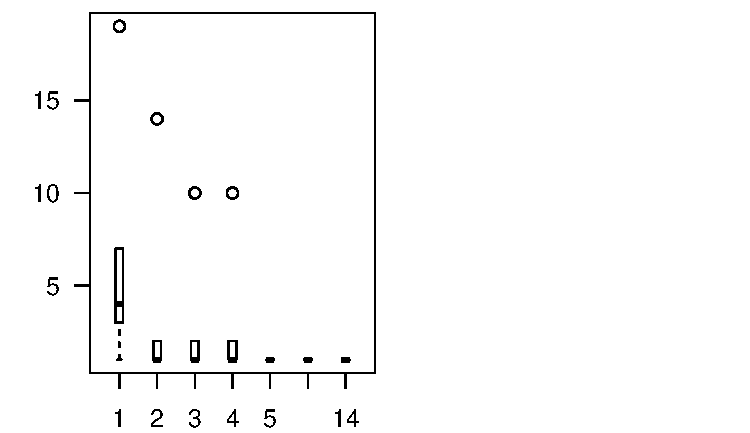
\includegraphics[scale=0.4,trim=20 0 130 0,clip]{R/idqaccess/idqaccess.pdf}
    \caption{idqaccess}
  \end{subfigure}%
  \begin{subfigure}{.2\textwidth}
    \centering
    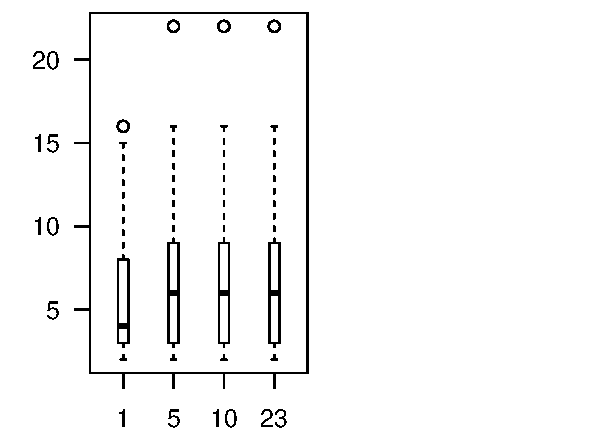
\includegraphics[scale=0.4,trim=15 0 130 0,clip]{R/scripttag/scripttag.pdf}
    \caption{scripttag}    
  \end{subfigure}%
\caption{Impact of number of positive examples.}
\label{fig:impact-number-attacks}
\end{figure}

\Mar{coloquem os numeros aqui para que eu gere o boxplot amanha,
  depois da aula. 

  *** posicao no ranking (numeros artificais. por favor, substituam) ***

  ataque 1:

    1 variacao:  10, 20, 4, 2, 5

    5 variacoes: 5, 4, 4, 2, 3

    10 variacoes: 1, 2, 1, 2, 1

    (ate numero de variacoes que aparece na Tabela 3)

    
  ataque 2:
     ...

}

%% \pgfplotsset{
%%   box plot width/.initial=0.5em
%% }
%% \begin{tikzpicture}
%%   \begin{axis}
%%     [
%%     ytick={1,2,3},
%%     yticklabels={Index 0, Index 1, Index 2},
%%     ]
%%     \addplot+[
%%     boxplot prepared={
%%       median=1,
%%       upper quartile=1.2,
%%       lower quartile=0.4,
%%       upper whisker=1.5,
%%       lower whisker=0.2
%%     },
%%     ] coordinates {};
%%     \addplot+[
%%     boxplot prepared={
%%       median=2,
%%       upper quartile=2.3,
%%       lower quartile=1.5,
%%       upper whisker=2.7,
%%       lower whisker=1
%%     },
%%     ] coordinates {};
%%     \addplot+[
%%     boxplot prepared={
%%       median=0.7,
%%       upper quartile=1.4,
%%       lower quartile=0.5,
%%       upper whisker=1.9,
%%       lower whisker=0.1
%%     },
%%     ] coordinates {};
%%   \end{axis}
%% \end{tikzpicture}


\subsection{Threats to Validity}
\label{sec:threats}

External Validity. \Fix{elaborate ...how popular are
  Suricata/Metasploit?}


\section{Discussion}

\subsection{Sample of other attacks}

\subsubsection{Remote Code Execution (RCE)}
\label{sec:rce}
\label{sec:jboss}
\label{sec:content-example}

%% Adaptacao do texto copiado de:  https://www.solarwindsmsp.com/blog/remote-code-execution

RCE refers to the family of attacks where hackers exploit a network
vulnerability to run arbitrary code---that could damage the system or
steal sensitive information---on a remote machine. JBoss~\cite{jboss}
is popular open source Java application server. This attacks enables
remote execution of code on the JBoss application server.
\Mar{@Lucas, por favor, observe o padrao usado nos exemplos
  anteriores. eh preciso explicar em alto nivel o ataque antes de
  explicar a regra!}

%% In an RCE attack, hackers
%% intentionally exploit a vulnerability in the system to run malware
%% By prompting the targeted device to perform code execution, a hacker
%% can run arbritrary code to
%% their own programming in its
%% place. This programming can then enable them to gain full access,
%% steal data, carry out a full distributed denial of service (DDoS)
%% attack, destroy files and infrastructure, or engage in illegal
%% activity. And as the term remote execution suggests, an RCE
%% cyberattack can take place from any geophysical location."\\


\begin{figure}[H]
  \lstinputlisting[language=C,numbers=none,keywords={content,flow}]{adaptor-golden-rule.suricata}
  \caption{\label{fig:rule-jboss}Suricata rule for JBoss Remote Code Execution.}
\end{figure}

%A opção  define que o match só será feito em pacotes que fazem parte
%de uma conexão já estabelecida entre um cliente e um servidor. Além
%disso, define também que os pacotes devem estar direcionados ao servidor, não ao cliente.

Figure~\ref{fig:rule-jboss} shows a Suricata rule that captures a
JBoss RCE attack.  The option \CodeIn{flow: established, to\_server;}
indicates that a rule match will only occur on packets that (1) flow
on an already-established connection and that (2) flow to the server
as opposed to the client. For the content options the modifiers
\CodeIn{nocase} and \CodeIn{http\_uri} indicate, respectively, that
the matching not be case sensitive and that the string should be
located at the packet field ``Request URI''. \Mar{Lucas, ``nocase''
  tambem eh considerado modificador? Isto nao eh confuso? Na secao
  4.3.4 consideramos modificadores como sinonimo para qualificador de
  campo, nao?}\Luc{Sim, ``nocase'' define que a busca pela string nao deve ser case sensitive. Em 4.3.4 estamos considerando apenas os modificadores que definem posições/campos de pacotes http.}

\tname{} reproduces the malicious JBoss attack using the traffic from
a Nikto script~\cite{nikto}. However, similar JBoss attack is also
available from the Metasploit database~\cite{metasploit}. As in the
other examples, \tname{} uses, as additional inputs, benign traffic
from \Fix{...} and a set of existing Suricata rules from
\Fix{...}. \tname{} initially produces one seed rule containing
\Fix{xx} options, by analyzing the malicious traffic alone. Then, it
uses that seed rule to derive \Fix{yy} rules, each rule containing
subsets of the option in the initial rule. Finally, it ranks that
list. The list below shows the top-5 rules that \tname{}
produces.\Mar{<- check/revise}

\Fix{list rules}

Note that the golden rule is in position \Fix{...} on this
case. \Mar{explain syntactical difference, if exist}

\subsubsection{Denial-of-Service}
\label{sec:dos}

\Mar{move from above --> We used the following hping3 command to
  reproduce that attack: \CodeIn{hping3 -d 80 -w 512 -S -p 80 --flood
    --rand-source <IP>}.}

The SYN Flood attack is a denial-of-service attack that exploits a vulnerability in the TCP/IP handshake
to establish a TCP connection~\cite{cloudfare-synflood}. The handshake
works as follows in normal circumstances. First, a client sends a SYN
packet to the server, requesting a connection. Second, the server
responds with a SYN-ACK packet to the client. Third, the client
responds with an ACK message and the connection is established. Aware
of the protocol, an attacker sends multiple SYN packets to different
ports of a server, often using fake IP addresses. Then, after the
server responds with a SYN-ACK packet, the client keeps sending other
SYN packets to avoid the connection to time out. Without proper
protection, the server accepts these malicious requests and eventually
legitimate requests cannot be satisfied due to resource exhaustion.

\vspace{-1ex}
\begin{figure}[h!]
  \lstinputlisting[language=C,numbers=none,keywords={flags,threshold}]{synflood.suricata}
  \vspace{-2ex}
  \caption{\suri\ rule for SYN Flood attack.}
  \label{fig:synflood-example}
\end{figure}
\vspace{-2ex}

Figure~\ref{fig:synflood-example} shows a Suricata rule that captures
this attack. This rule was obtained from the Emerging Threats Open
Ruleset~\cite{emerging-threats-open}. The relevant options in the
rule appear in bold---the option \CodeIn{flags: S,12}, identifies a
SYN packet in a TCP packet and the option \CodeIn{threshold: type
  both, track by\_dst, count 5000, seconds 5} indicates that a high
volume of such packets should be requested in a short period of
time. The other options are for documentation purposes.


...........
In this case, however, that information alone is
insufficient as the malicious traffic is characterized as a sequence
of messages. 
...........


%% \Mar{...and where did they come from?} \Luc{Sim, floods podem ser
%% compostos por milhares de pacotes, um dos data sets q encontrei
%% possui mais de 500k pacotes de flood. Os data set  s foram encontrados na internet.}

\begin{figure}[h]
  \vspace{-2ex}
  \lstinputlisting[language=C,numbers=none,frame=none,keywords={flags,threshold,window}]{synflood.suricata.synth}
%  \caption{Suricata rule for SYN Flood Attacks.}
  %  \label{fig:synflood-example-synt}
  \vspace{-2ex}  
\end{figure}

%% \Mar{@Lucas/Guilheme, há algo o que remover? talvez ``window:64''?
%%   Qual a correspondencia de ``flags:S,12'' com ``flags:S''? Por favor,
%%   respondam isto logo.}  \Gui{O window:64 seria removido
%%   sim.}\Mar{ok. vou explicar isto.}
  %% \Luc{O segundo campo da opção flags define flags que serão
  %%   ignoradas. Nesse caso a regra procura por pacotes onde apenas a
  %%   flag S está 'setada', independentemente do valor das flags 1 e
  %%   2. Portanto a regra gerada pode capturar coisas diferentes da
  %%   regra original. A inferencia do "12" n pode ser feita apenas a
  %%   partir do pacote de entrada, precisariamos tratar
  %%   isso.}\Mar{vc. pode explicar isto **mais detalhadamente** \Luc{a opção flags pode ter dois campos separados por virgula (ex: flags:S,12). o primeiro campo indica quais flags devem estar ativas em um pacote para que o suricata gere um alerta. se uma ou mais flags forem irrelevantes para a detecção de um determinado ataque (ou seja, se n importa se a flag está ou não ativa), elas serão adicionadas ao segundo campo.} E (1)
  %%   explicar que isto eh uma limitacao \Luc{n entendi exatamente oq explicar aqui.} e (2) indicar a possivel consequencia
  %%   disto? \Luc{a consequencia sao possiveis falsos negativos. ao não incluir flags no segundo campo podemos descartar pacotes por conta da presença de flags q n são relevantes (ou seja, vamos levar em conta flags q n deveriam interferir na detecção).}}

\noindent

.....

 The list below shows the rule options for the top-5 rules
\tname{} produces for this attack.\Mar{algum problema em fazer isto?
  exemplos concretos ajudam muito!} \Luc{No caso desse ataque, a regra inicial possui apenas duas opcoes (sem contar o threshold). Entao existem apenas 3 combinacoes possiveis, dessas 3 apenas 2 sao capazes de isolar o ataque do trafego normal. Portanto, o top-2 eh:
  \begin{figure}[h]
    \vspace{-2ex}
    \lstinputlisting[language=C,numbers=none,frame=none,keywords={window,flags}]{top-synflood.rules}
    \vspace{-3ex}  
  \end{figure}

   }\Mar{Lucas, eu nao entendo porque vc. desconsiderou threshold da
  discussao (afinal, a gente destaca thrshold como relevante no inicio
  desta secao). tambem nao entendo porque window---que a gente disse
  acima que *nao* era relevante---aparece nas duas regras
  geradas. enfim, isto esta inconsistente com nosso discurso.}

\vspace{1ex}
\noindent
\textbf{Differences.}~Note that there are differences between the
options produced in the first step of \tname{} and the options from
the golden rule, as per Figure~\ref{fig:synflood-example}. The option
\CodeIn{flags} does not mention parameters \CodeIn{1 2}, there is an
extra option \CodeIn{window}, and there are differences in the option
\CodeIn{threshold}. Considering the option \CodeIn{flags}, the first
parameter of that option indicates what flags in the packet must be
set while the second parameter indicates non-mandatory flags (\ie{},
``don't cares''). More specifically, the option \CodeIn{flags: S}
indicates that the flag ``S'' must be set and all flags not mentioned
(including ``1'' and ``2'') must be unset for the \nids\ to capture
the traffic. Consequently, that choice of option alone could result in
false negatives and false positives. An attack that satisfies all
other conditions in a rule and has flags ``1'' or ``2'' set would be
captured by the original rule but not captured by the inferred rule---a case of
false negative. Likewise, an attack that satisfies all conditions and
have flags ``1'' and ``2'' unset would be captured by the inferred
rule but not captured by the original rule---a case of false positive. The set of
positive examples is to blame in this case. To mitigate this issue,
the input messages should have covered cases with options ``1'' or
``2'' set. Considering option \CodeIn{window: 512}, \tname{} is able
to generate rules without that option, as discussed above. Considering
option \CodeIn{threshold}, the values used in the golden rule are
domain-specific. \tname{} uses default values for these options. We
conjecture that the system administrator would be able to configure
this option.


%% \begin{table}[h]
%%   \caption{\label{table:rules}Rule evolution}  
%%   \centering
%%   \begin{tabular}{lllll}
%%     \toprule
%%     \multicolumn{1}{c}{Iteration} & \multicolumn{1}{c}{Rule} \\
%%     \midrule     
%%     0 & (ack:0; seq:0; window:0; flags:F;)\\
%%     5 & (window:0; flags:F;)\\
%%     68 & (window:64; flags:F;)\\
%%     73 & (window:64; flags:S,12;)\\
%%     94 & (window:64; flags:S,12; threshold: type both, track by\_dst, count 20, seconds 1;)\\
%%     \bottomrule
%%   \end{tabular}
%% \end{table}



\section{Related Work}

\Fix{...}

\section{Conclusions}

\Fix{...}

%% \section*{Acknowledgments}
%% This work is partially supported by RNP grant number 002951.

\balance
\bibliographystyle{ACM-Reference-Format}
\bibliography{references}

\end{document}
\endinput
%%
%% End of file `sample-sigconf.tex'.
